\subsection{Description of the Structures in the Increasing Archetypal Model}
\label{sec:add.add.like}

The first step in the description of the \gls{pal} structures is plotting a 2D scan of the periods of such a structure.
Here, $b_L$ is changed to $0.8$, and $a_L$ and $g_R\left(\frac{1}{2}\right)$ are kept as described before, because the \gls{pal} structures are more pronounced at these parameter values.
\Cref{fig:add.add.like} shows a 2D period scan with these parameters at a corner of the space between chains.
Here, the parameter region $P^{12}_2$ is in the lower left corner and the parameter region $P^{12}_3$ of the same chain is in the upper right corner.
In the lower right corner is the parameter region $P^{14}_3$.

Next, this section takes a closer look at the horizontally \gls{pal} structures between the parameter regions $P^{14}_3$ and $P^{12}_3$.
After that, it examines the vertically oriented \gls{pal} structures between the parameter regions $P^{12}_2$ and $P^{14}_3$.
And lastly, it examines the complex looking structure in the corner between all three ``type A'' parameter regions.

\begin{figure}
	\centering
	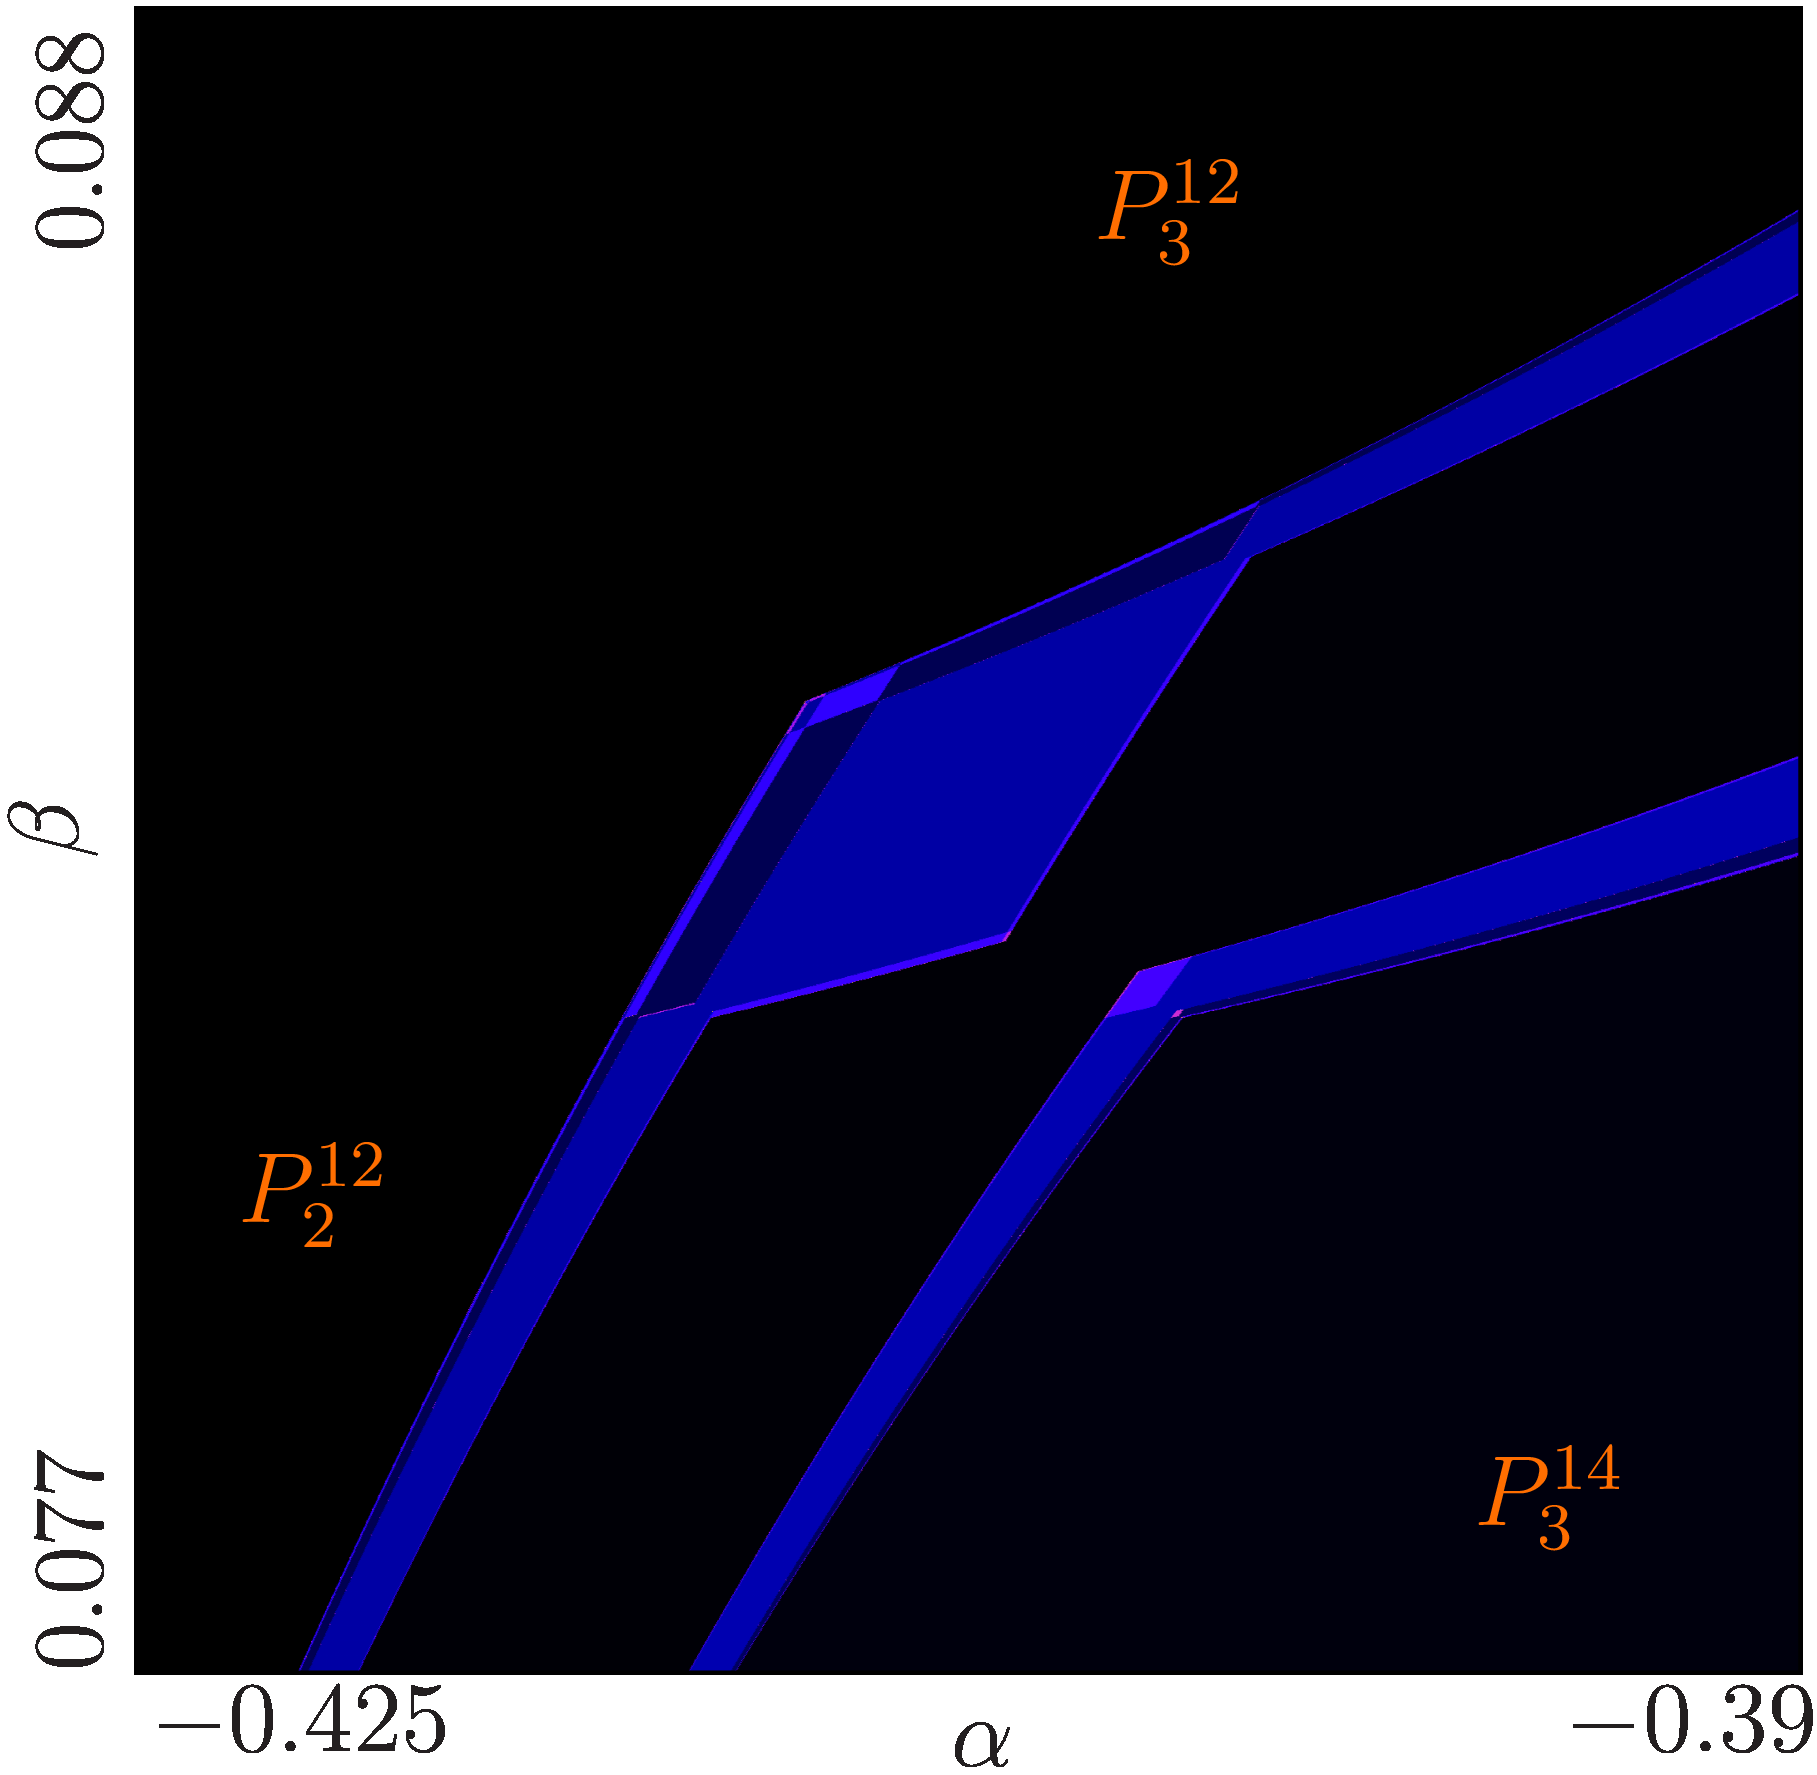
\includegraphics[width=.7 \textwidth]{../Figures/7/7.11/result.png}
	\caption[2D period scan of period-adding-like structures in the increasing archetypal model]{
		2D period scan of period-adding-like structures in the increasing archetypal model.
		The fixed parameters are $a_L = 1, b_L = 0.8,$ and $g_R\left(\frac{1}{2}\right) = \frac{1}{2} + \frac{1}{40}$.
		The parameters $\alpha = g_R\left(\frac{1}{4}\right)$ and $\beta = c_L$ are varied.
	}
	\label{fig:add.add.like}
\end{figure}

\subsubsection{Horizontal Period-adding-like Structures}

\Cref{fig:add.add.like.hor.2D} shows a 2D scan of the horizontally oriented \gls{pal} structures between the parameter regions $P^{14}_3$ and $P^{12}_3$.
We can see two \gls{pal} structures, one between the ``type A'' parameter region $P^{14}_3$ and the hybrid parameter region $\left[P^{14}_3 \mid P^{12}_3\right]$ and one in between the hybrid parameter region $\left[P^{14}_3 \mid P^{12}_3\right]$ and the ``type A'' parameter region $P^{12}_3$.
There is a red arrow in the 2D period scan that indicates the parameter range for the 1D period scan in \Cref{fig:add.add.like.hor.1D}.

Looking at the 1D period scan, one can see why the section is called \glsentrylong{pal}.
In the middle between the parameter regions associated with the periods $14$ and $13$, we would expect the most pronounced parameter region to be associated with the period $27$.
Instead, the most pronounced parameter region in-between those parameter regions is associated with the period $40$.
And the most pronounced parameter region between this parameter region and the parameter region associated with the period $14$, has period $27$ where we would expect period $54$.
We can see that the periods do not add in our case.

\begin{figure}
	\centering
	\subfloat[2D period scan]{
		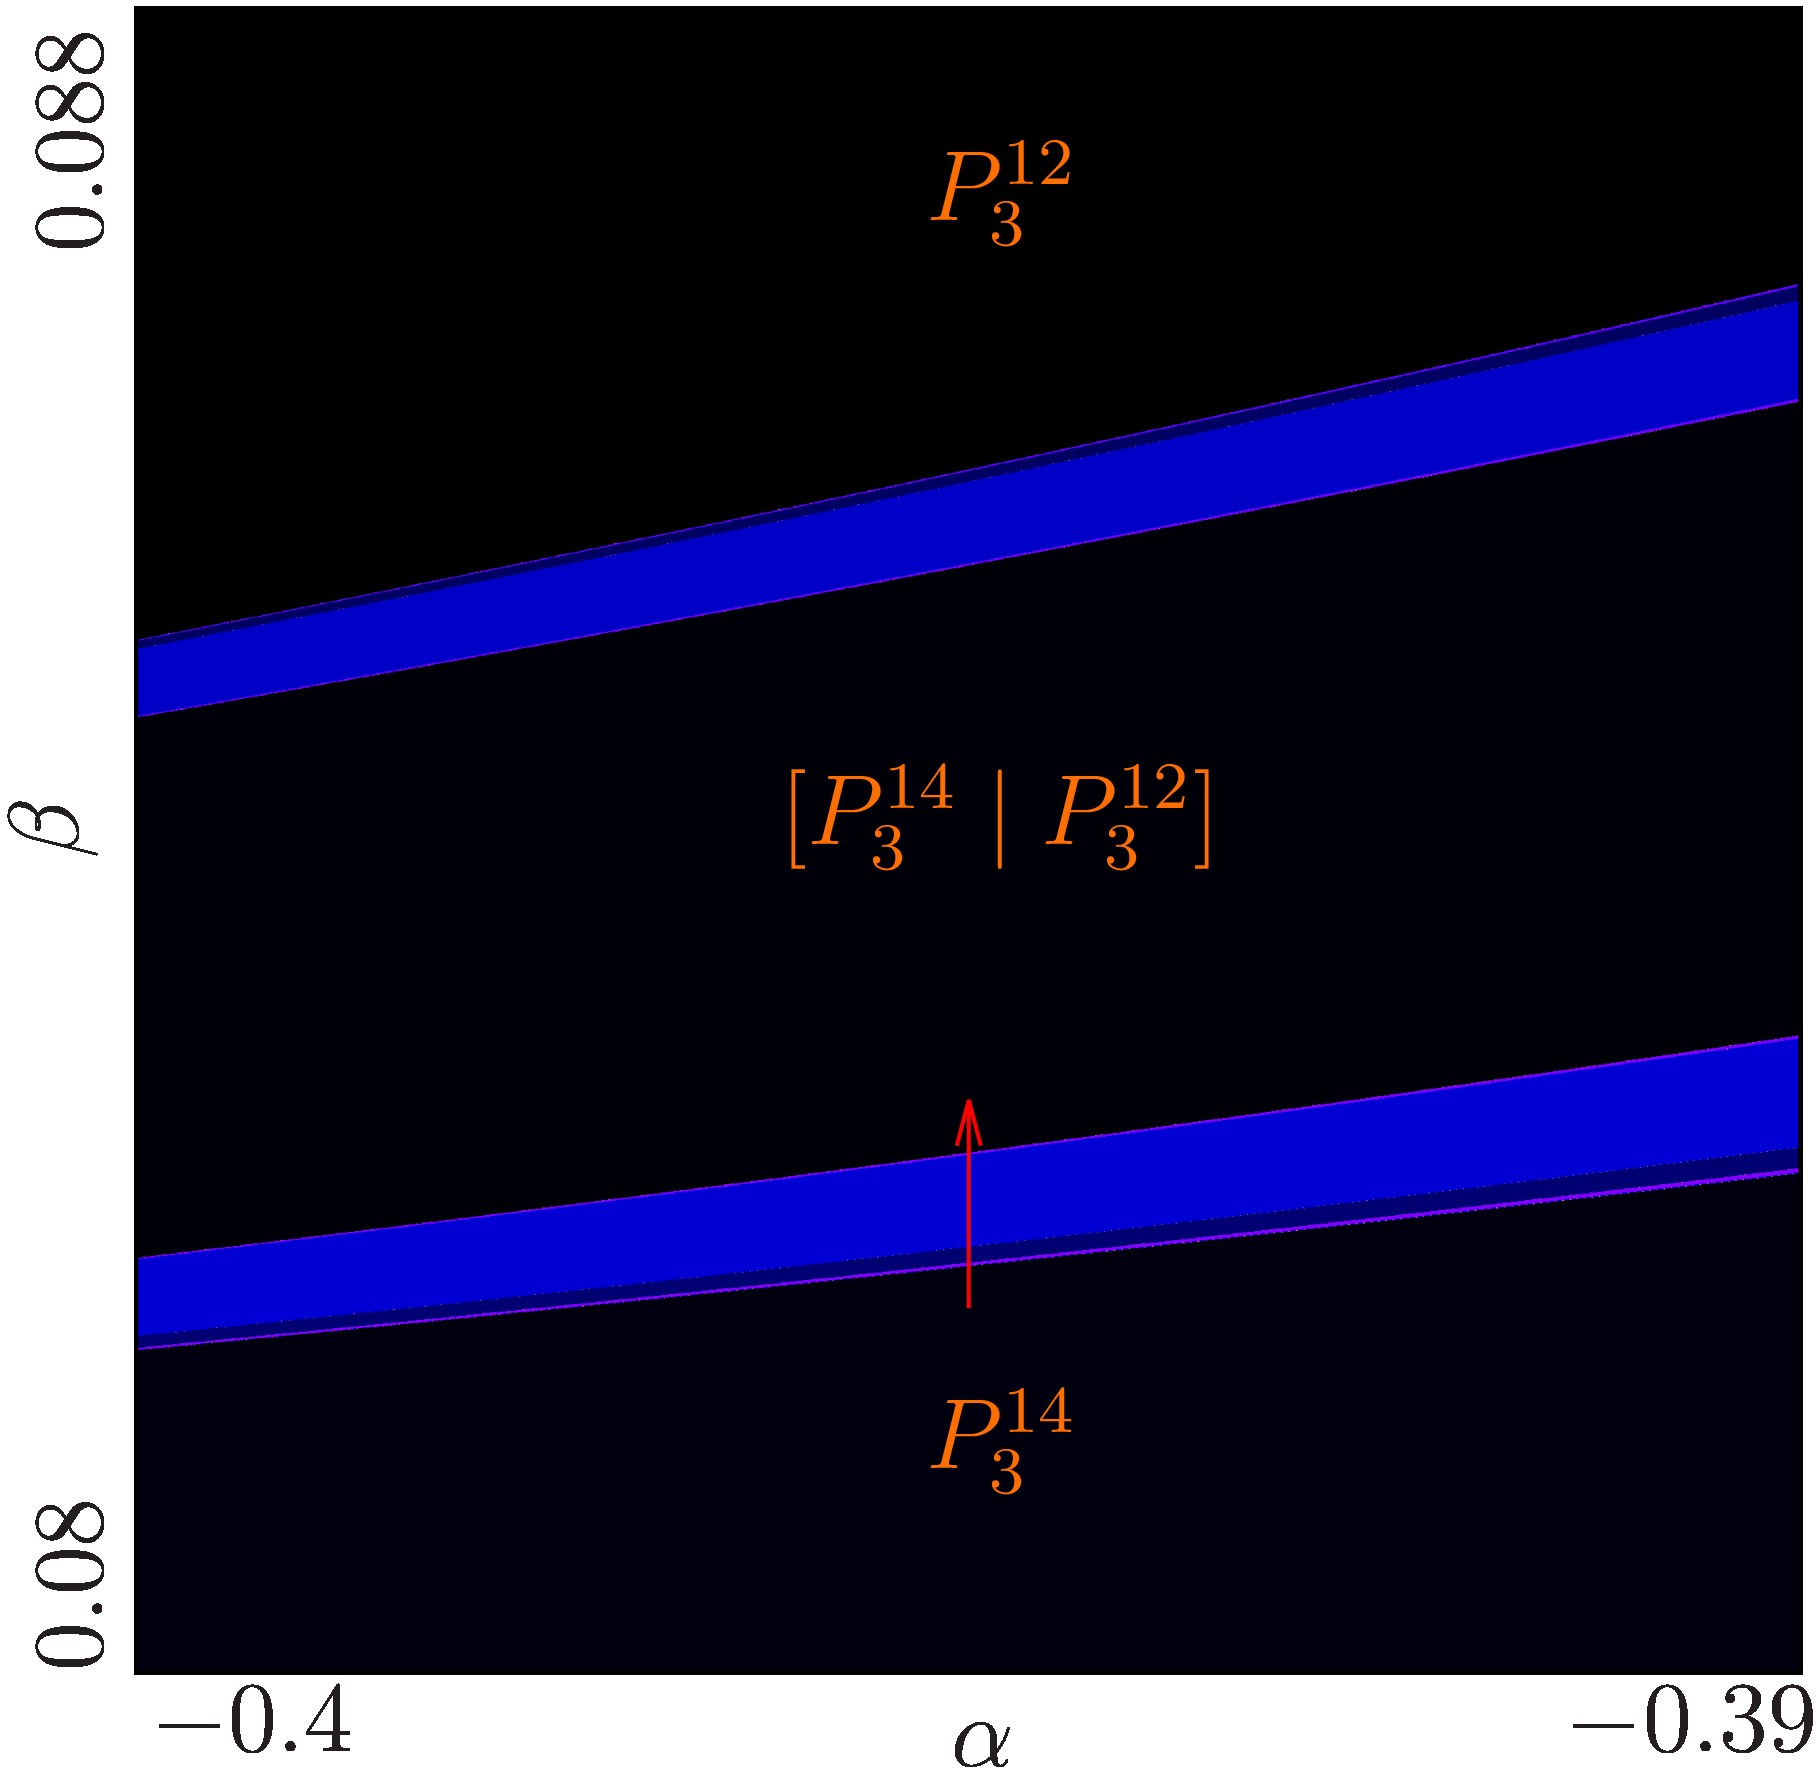
\includegraphics[width=.45 \textwidth]{../Figures/7/7.12a/result.png}
		\label{fig:add.add.like.hor.2D}
	}
	\subfloat[1D period scan]{
		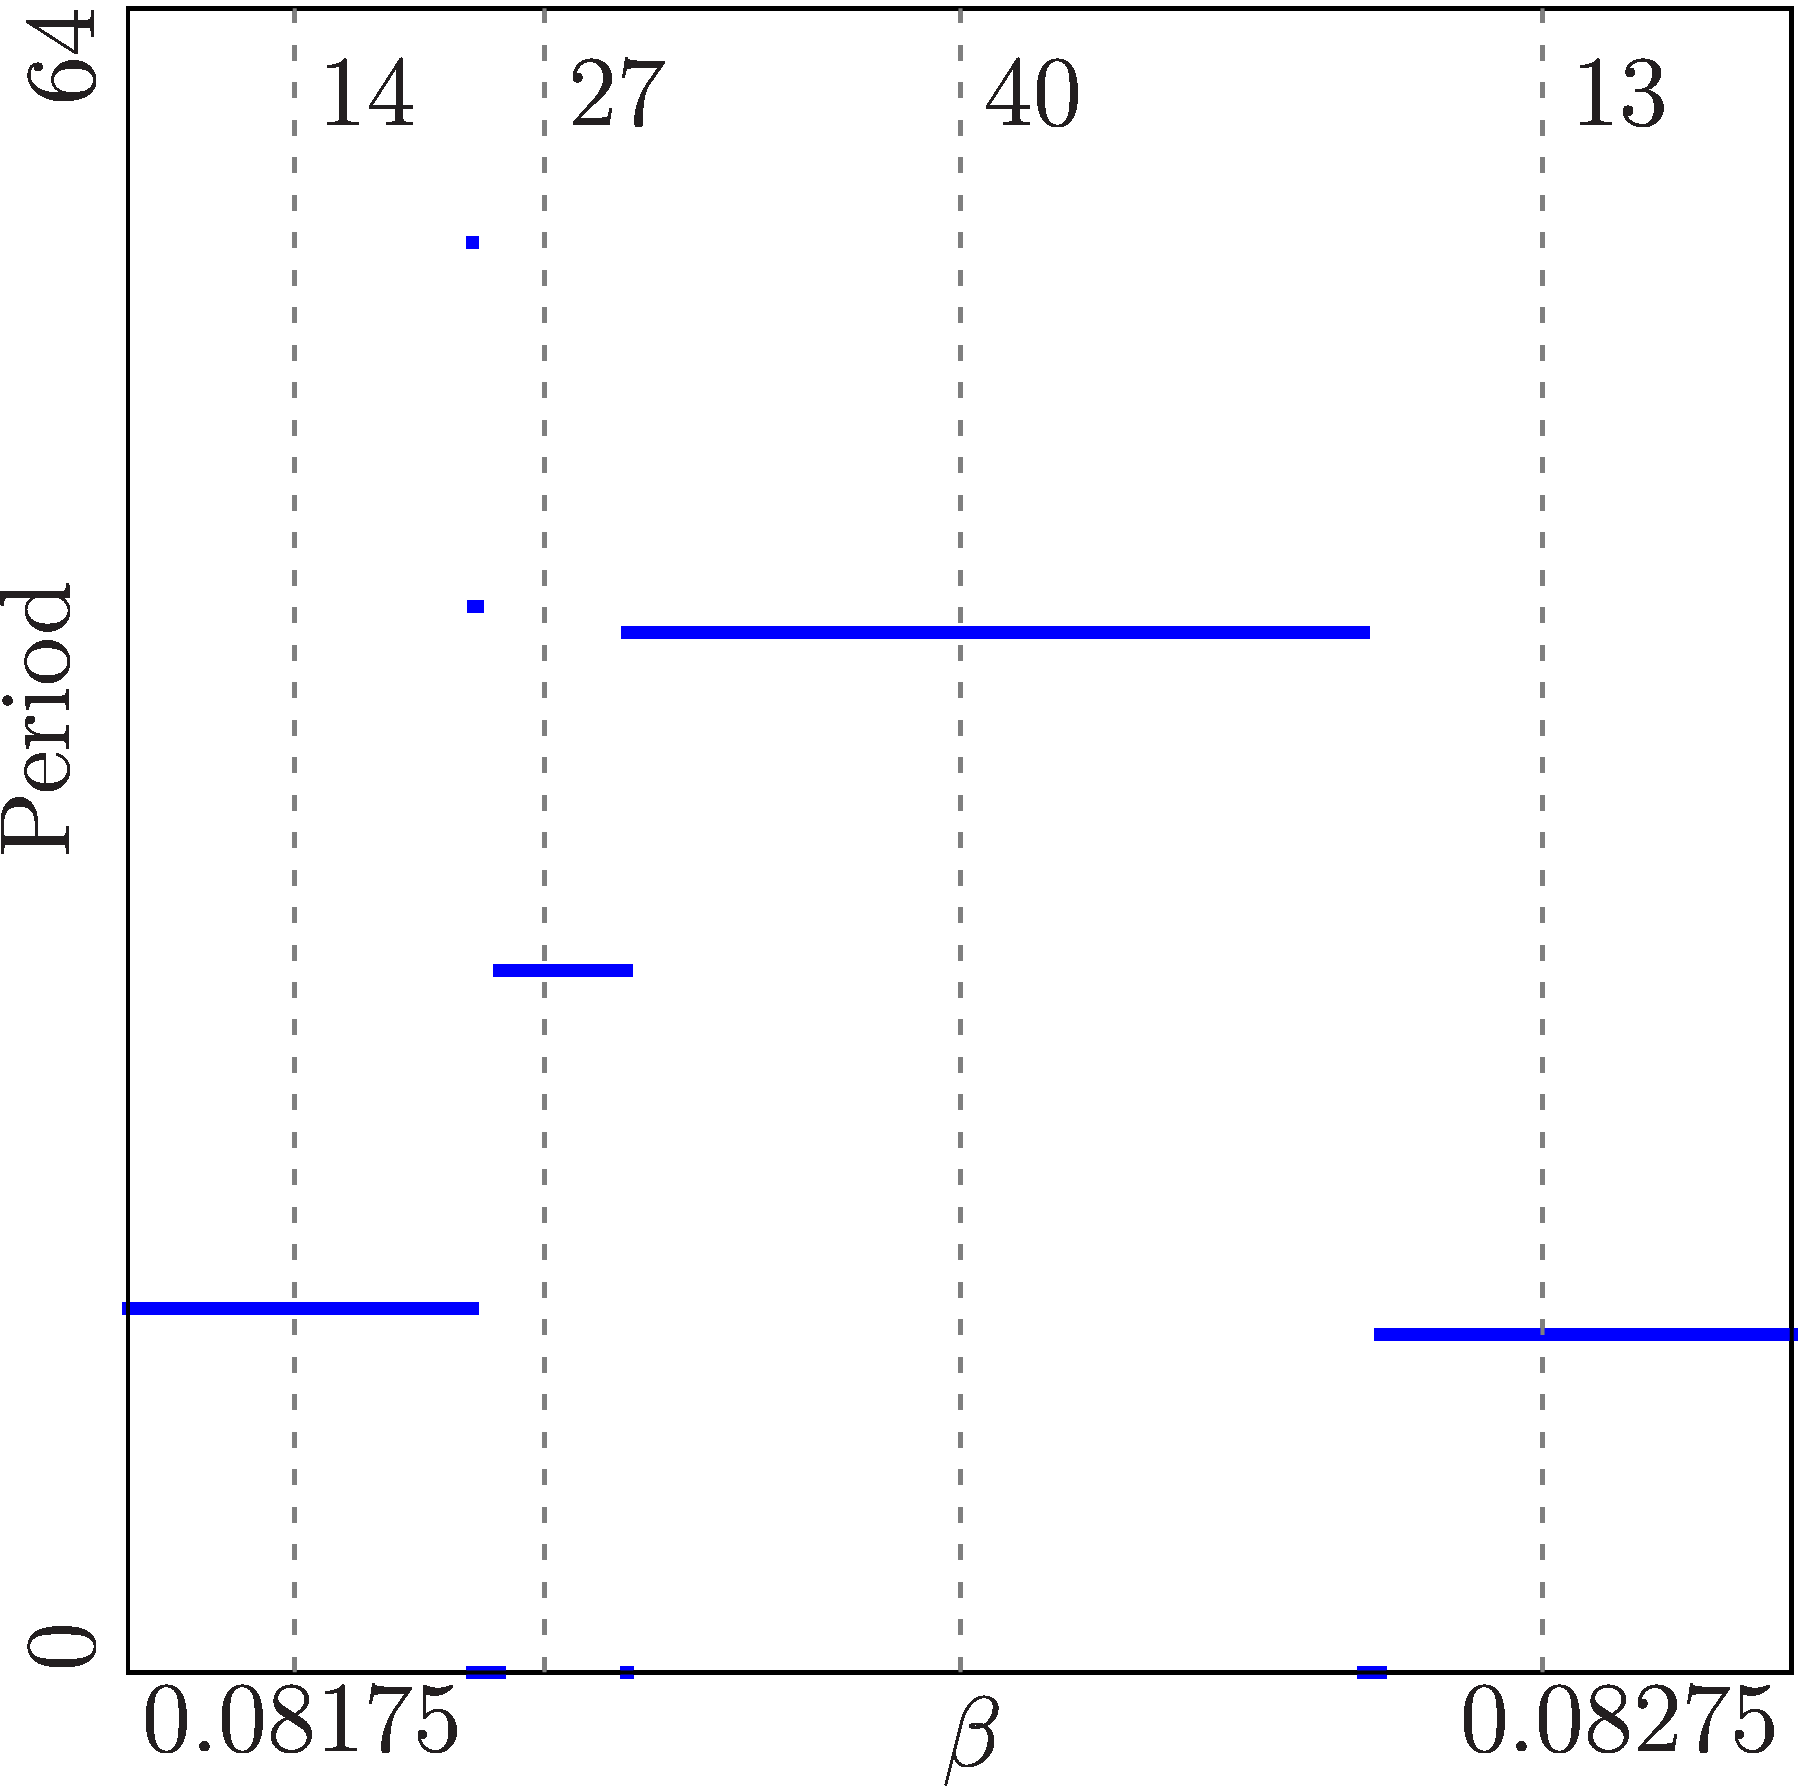
\includegraphics[width=.45 \textwidth]{../Figures/7/7.12b/result.png}
		\label{fig:add.add.like.hor.1D}
	}
	\caption[2D and 1D period scans of horizontal period-adding-like structures in the increasing archetypal model]{
		2D and 1D period scans of horizontal period-adding-like structures in the increasing archetypal model.
		The fixed parameters are $a_L = 1, b_L = 0.8,$ and $g_R\left(\frac{1}{2}\right) = \frac{1}{2} + \frac{1}{40}$.
		(a) shows the 2D period scan where the parameters $\alpha = g_R\left(\frac{1}{4}\right)$ and $\beta = c_L$ are varied.
		The small arrow indicates the parameter range for the 1D period scan in (b).
		Here, only $\beta$ is varied.
		The numbers at the top mark the periods at the corresponding value for $\beta$.
	}
	\label{fig:add.add.like.hor}
\end{figure}

The structure is not just a skewed \gls{pa} structure, as one might think since the period $27$ is associated with another parameter region that is not the most pronounced between the parameter regions associated with the periods $14$ and $13$, respectively.
And also $27 + 13 = 40$ which is associated with the parameter region between the parameter regions associated with the periods $27$ and $13$, respectively.
We can see that when examining the symbolic sequences associated with the parameter regions in that structure.
\Cref{fig:add.add.like.hor.tree} shows the Farey-tree with the symbolic sequences of this structure.
The starting nodes are associated with the symbolic sequences associated with the parameter regions $P^{14}_3$ and $\left[P^{14}_3 \mid P^{12}_3\right]$, respectively.
The parameter region associated with the period $27$ is the lowest node in level $2$, which is associated with two coexisting cycles.
These two cycles, $\A^4\B^3\C^4\D^3\A^4\B^3\C^3\D^3$ and $\A^4\B^3\C^4\D^3\A^3\B^3\C^4\D^3$ could be the result of concatenating the symbolic sequences $A^4\B^3\C^4\D^3$ and $\A^4\B^3\C^3\D^3$, as well as $\A^4\B^3\B^4\D^3$ and $\A^3\B^3\C^4\D^3$ of the parameter regions associated with the periods $14$ and $13$, respectively.
But the cycle $\A^4\B^3\C^4\D^3\A^3\B^3\B^4\D^3\A^4\B^3\C^3\D^3$ of the parameter region associated with the period $40$ cannot be a result of concatenating any pair of symbolic sequences $\A^4\B^3\C^3\D^3$ and $\A^3\B^3\C^4\D^3$ of the parameter region associated with the period $13$ and $\A^4\B^3\C^4\D^3\A^4\B^3\C^3\D^3$ and $\A^4\B^3\C^4\D^3\A^3\B^3\C^4\D^3$ of the parameter region associated with the period $27$.
One can see that this is truly no \gls{pa} structure.

\begin{figure}
	\centering
	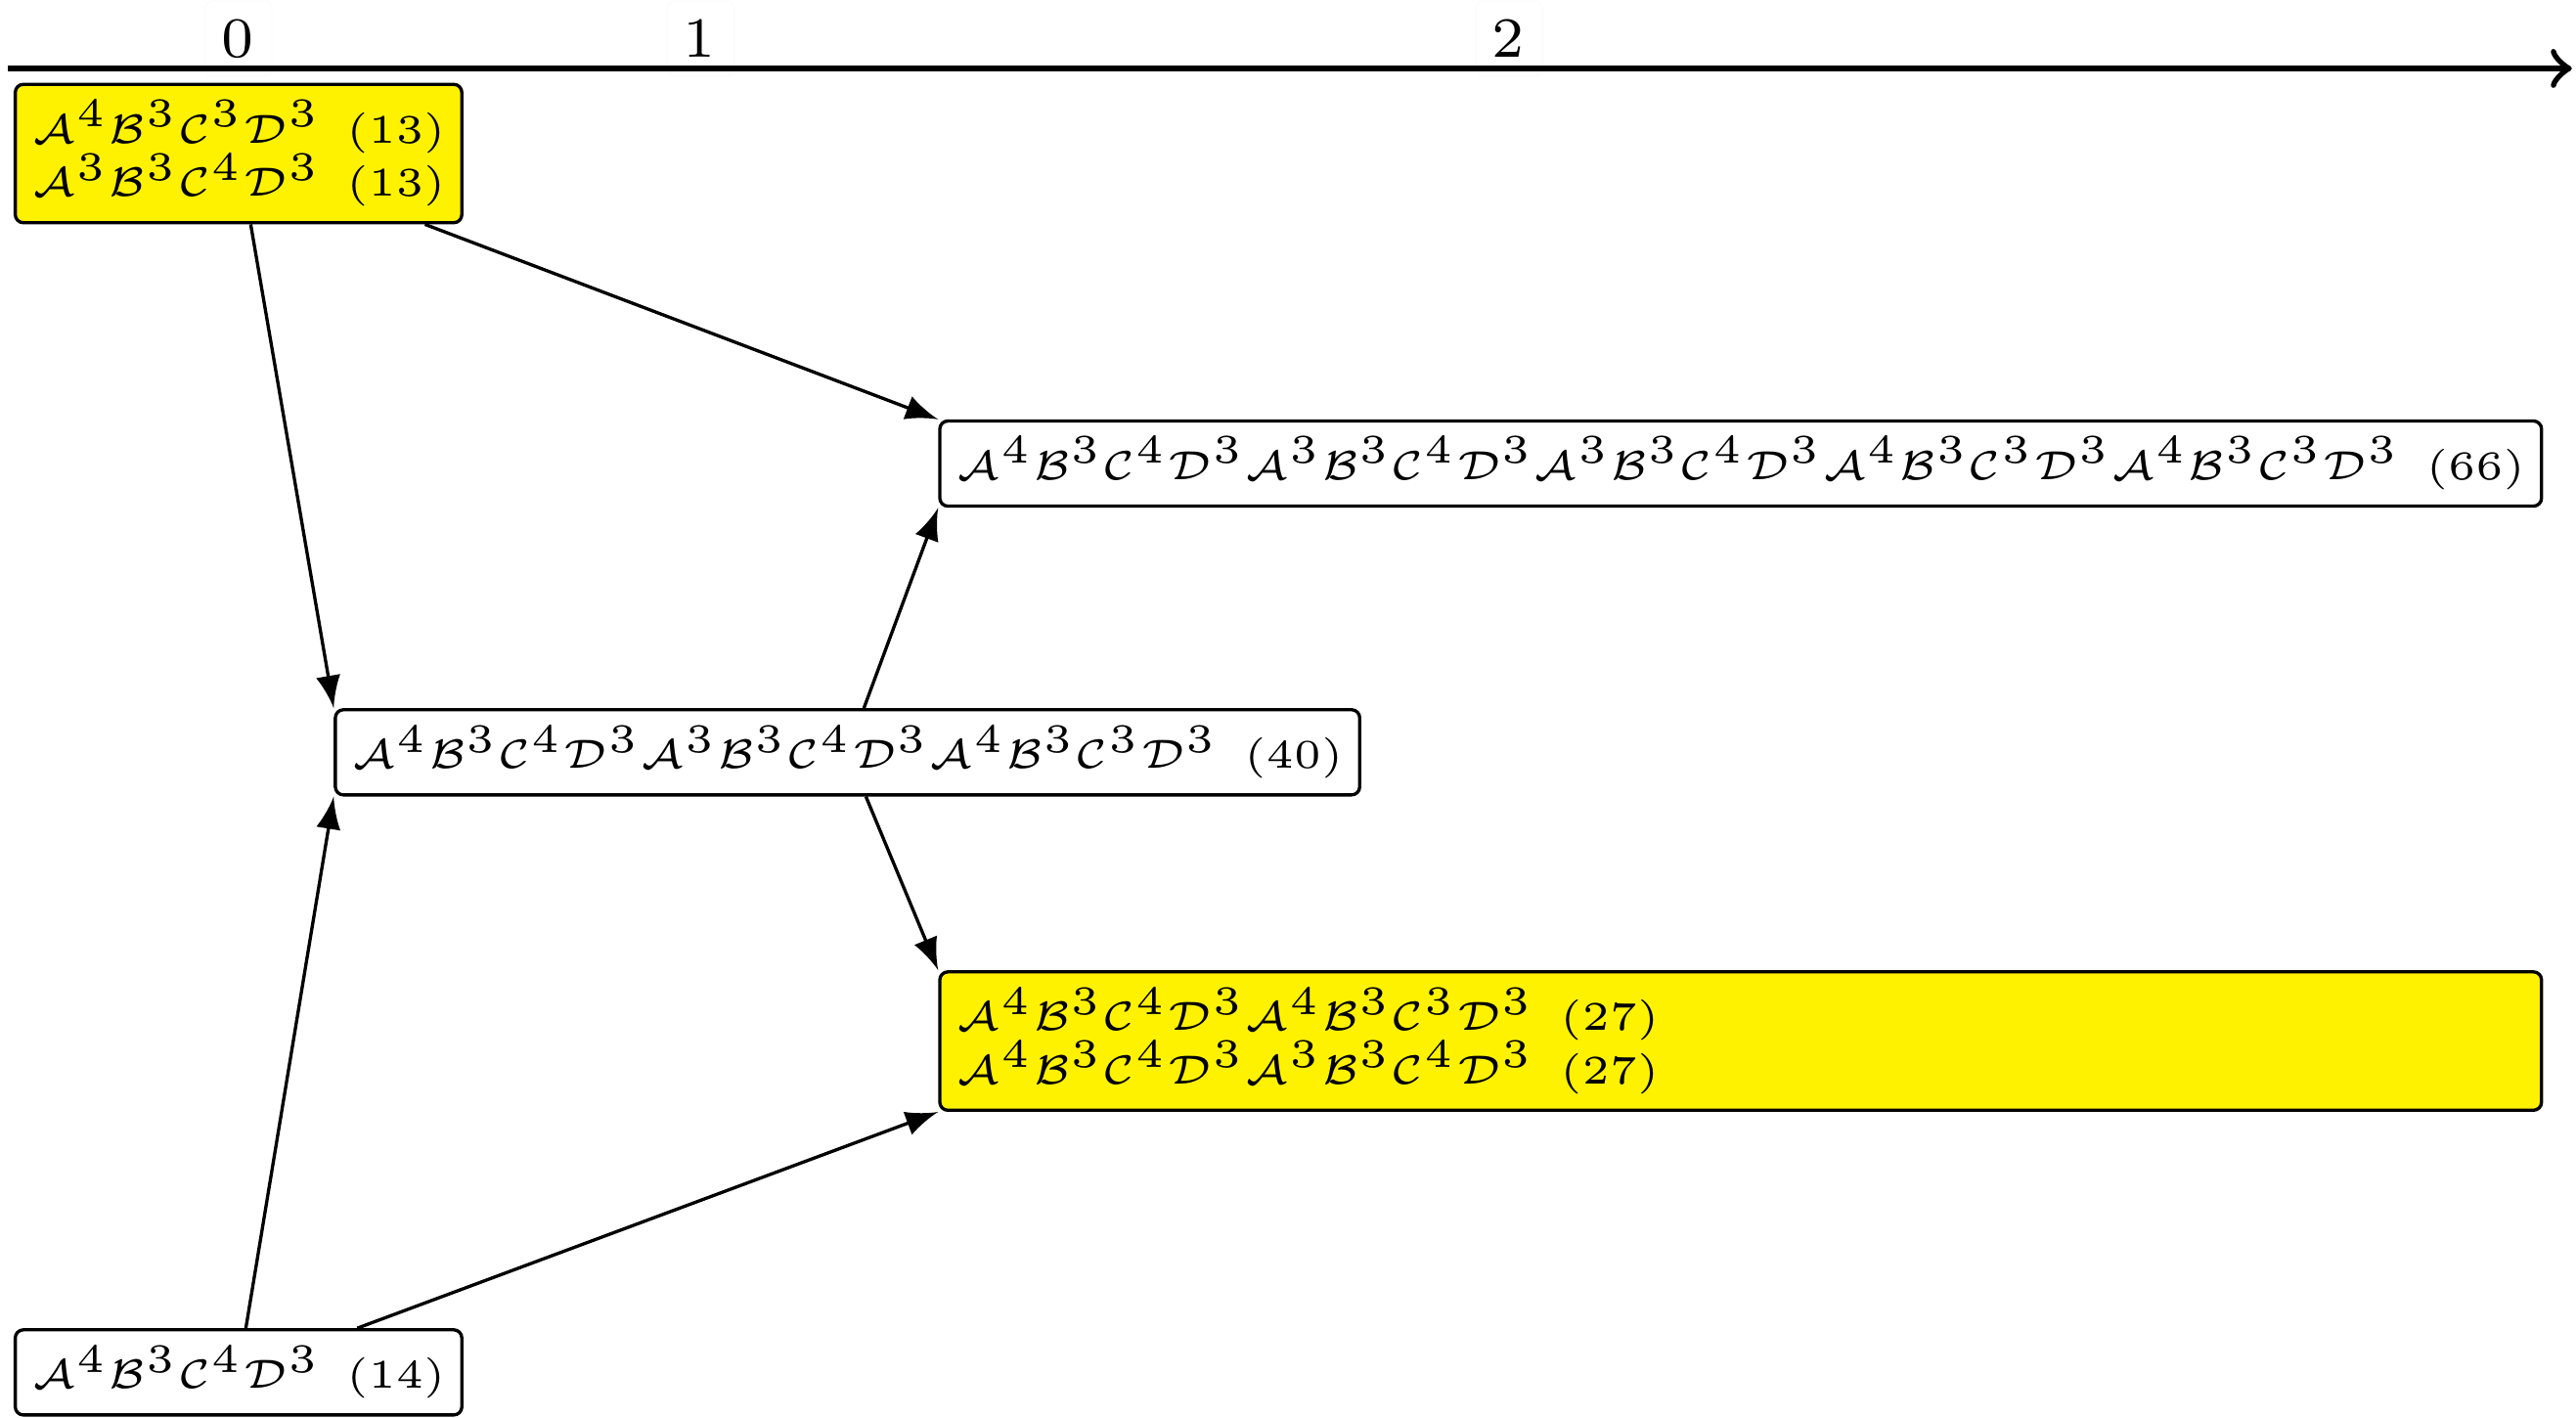
\includegraphics[width=.7 \textwidth]{../Figures/7/7.13/adding.png}
	\caption[Farey-tree with the symbolic sequences of a horizontal \glsentrylong{pal} structure]{
		Farey-tree with the symbolic sequences associated with the parameter regions of the lower horizontal \gls{pal} structure marked with a red arrow in \Cref{fig:add.add.like.hor.2D} up to two levels.
		Nodes of parameter regions associated with two coexisting cycles are colored yellow.
	}
	\label{fig:add.add.like.hor.tree}
\end{figure}

\subsubsection{Vertical Period-adding-like Structures}

Next, vertically oriented \gls{pal} structures are examined.
\Cref{fig:add.add.like.vert.2D} shows a 2D period scan of this structure.
Here, we can also see two \gls{pal} structures, one in-between the parameter regions $P^{12}_2$ and $\left[P^{12}_2 \mid P^{14}_3\right]$ and one in-between the parameter regions $\left[P^{12}_2 \mid P^{14}_3\right]$ and $P^{14}_3$.
The \gls{pal} structure in-between the parameter regions $P^{12}_2$ and $\left[P^{12}_2 \mid P^{14}_3\right]$ is chosen for closer investigation.
Again, a red arrow marks the parameter range for the 1D period scan of this \gls{pal} structure in \Cref{fig:add.add.like.vert.1D}.

As before, the periods do not add as we would expect from a \gls{pa} structure.
The most pronounced parameter region between the parameter regions associated with the periods $12$ and $13$ is associated with the period $38$.
And the most pronounced parameter region between this parameter region and the parameter region associated with the period $12$ is associated with the period $25$, which should have been the most pronounced parameter region between the parameter regions associated with the periods $12$ and $13$, respectively.

\begin{figure}
	\centering
	\subfloat[2D period scan]{
		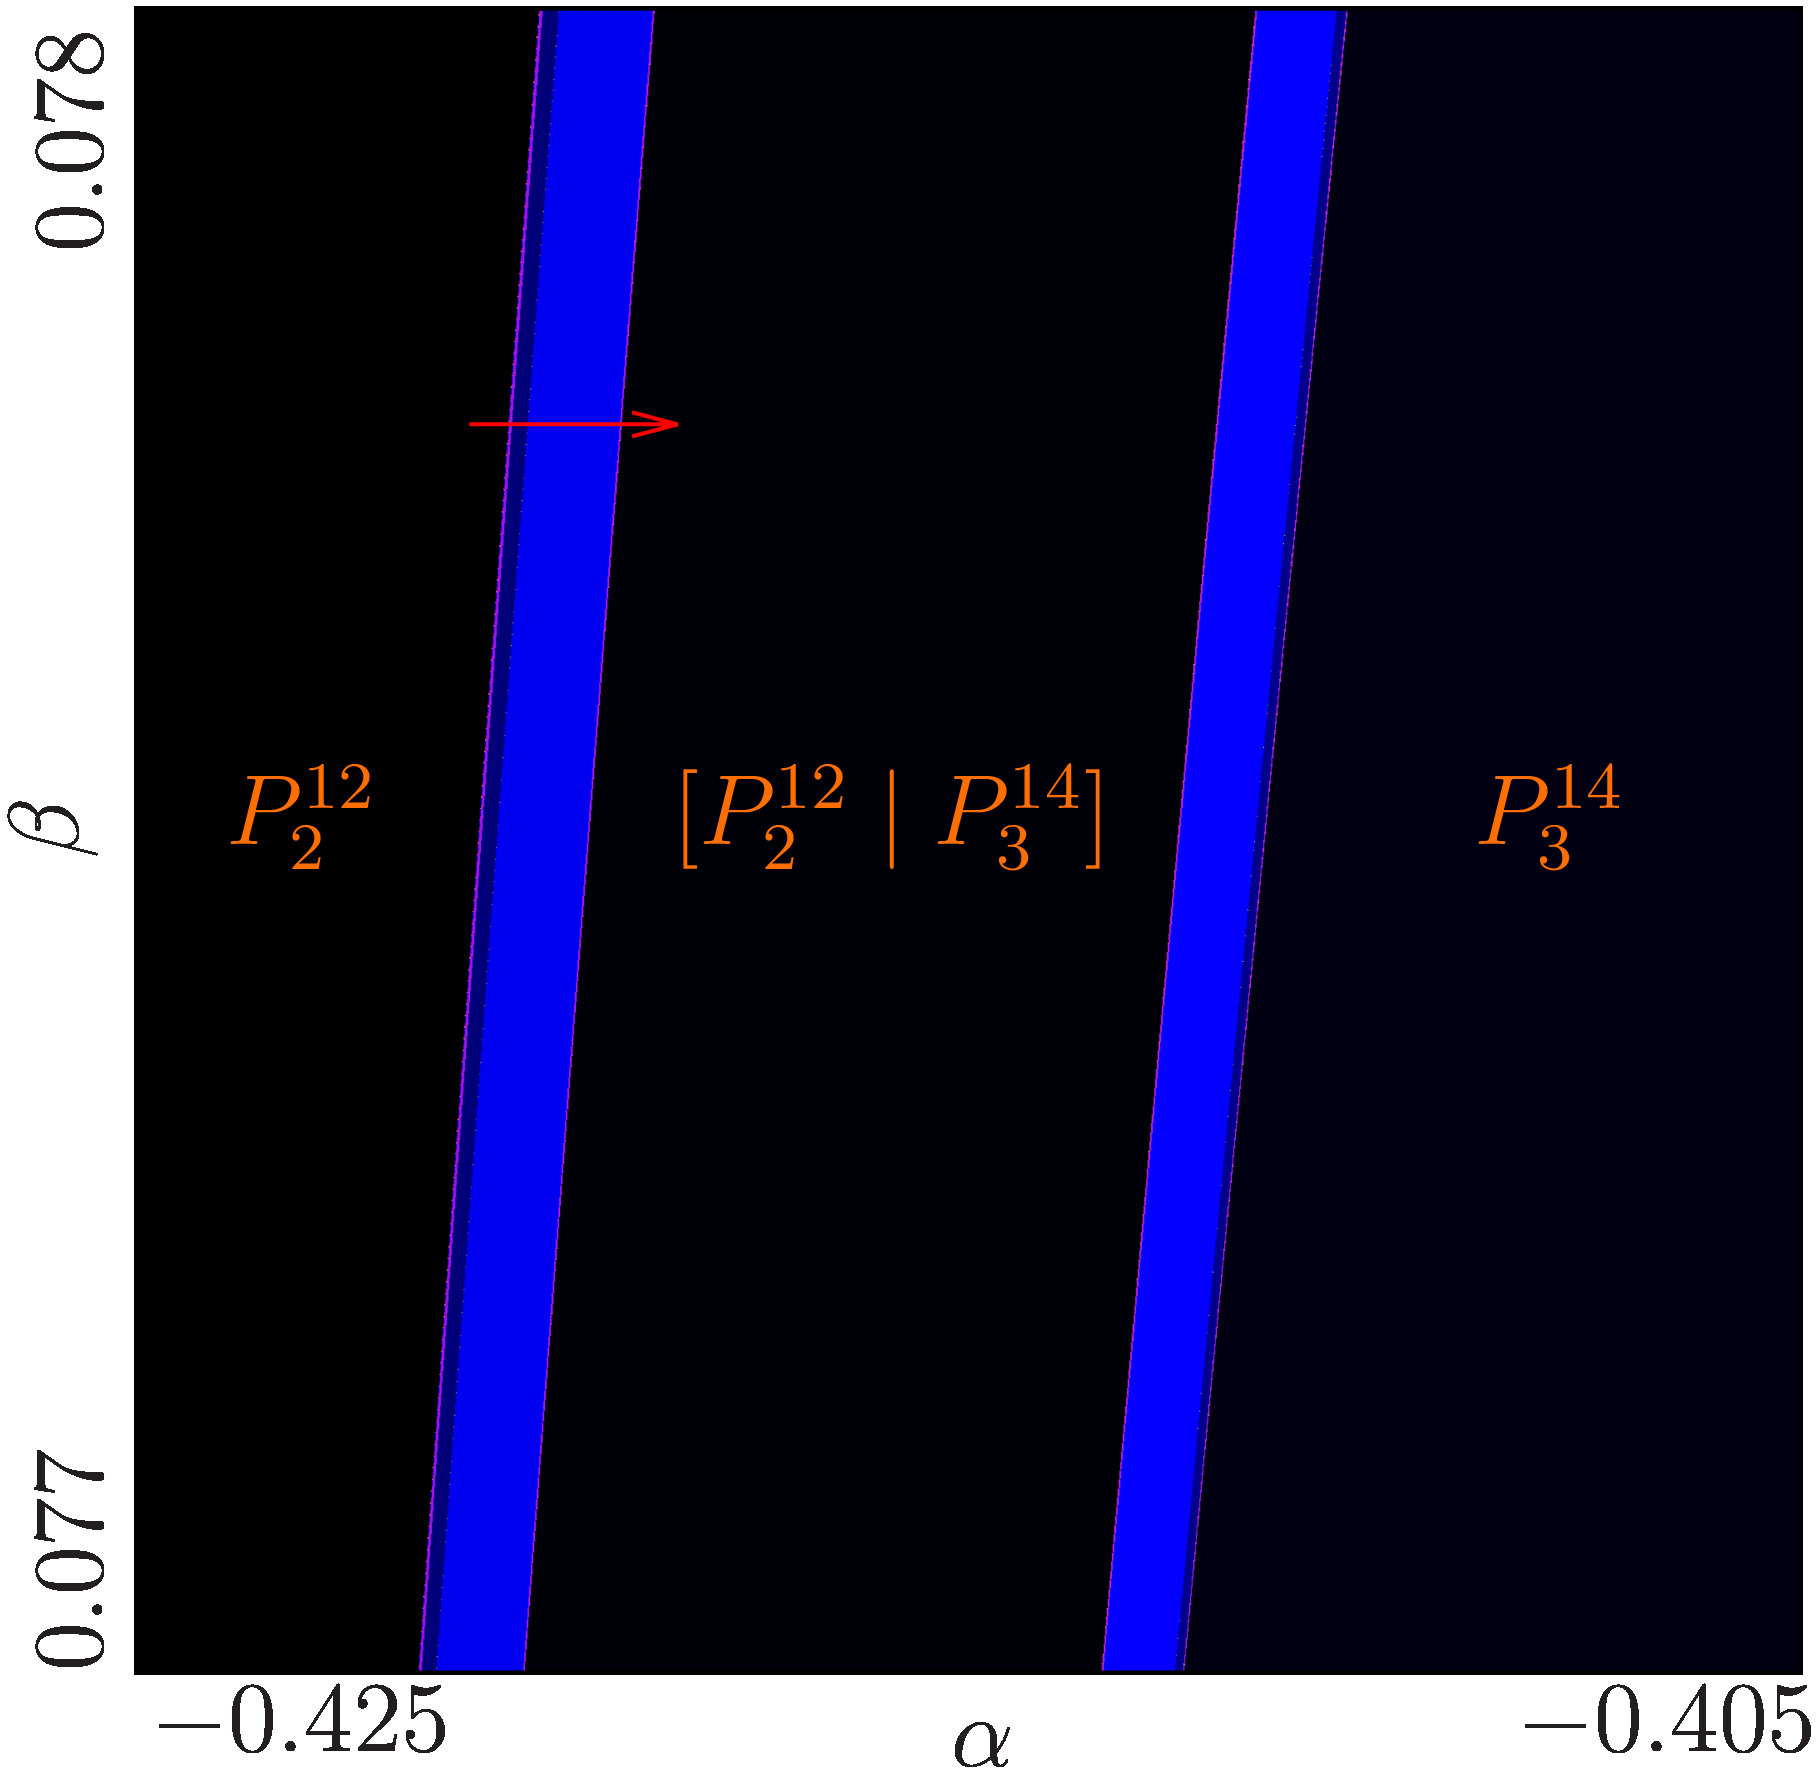
\includegraphics[width=.45 \textwidth]{../Figures/7/7.14a/result.png}
		\label{fig:add.add.like.vert.2D}
	}
	\subfloat[1D period scan]{
		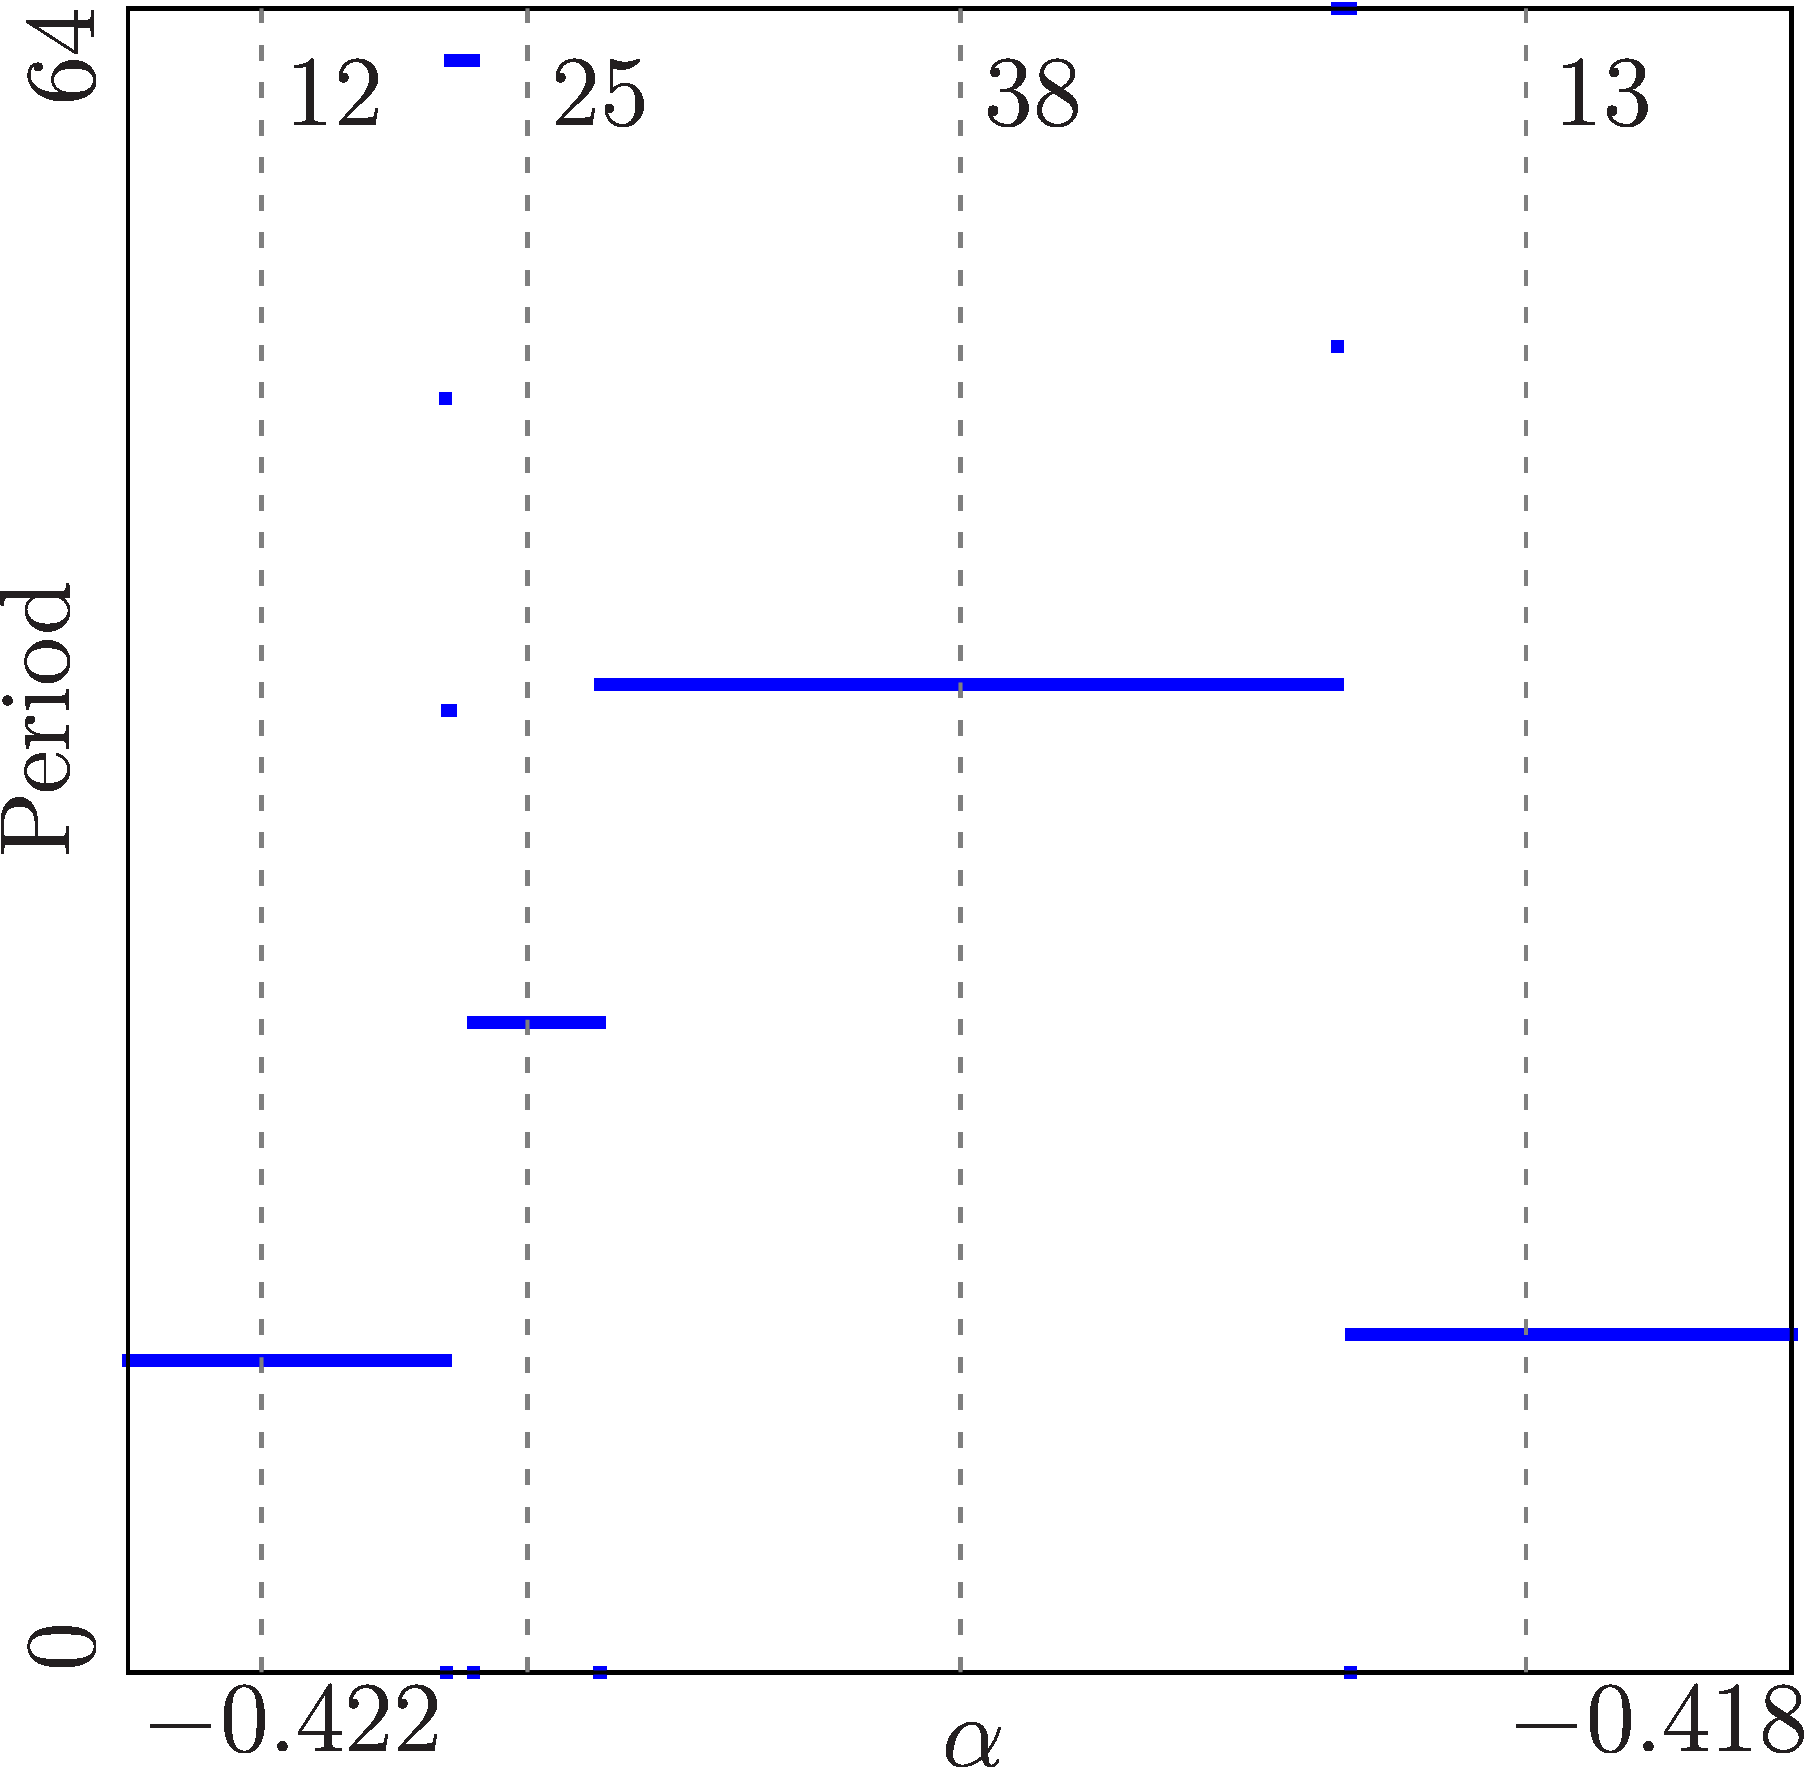
\includegraphics[width=.45 \textwidth]{../Figures/7/7.14b/result.png}
		\label{fig:add.add.like.vert.1D}
	}
	\caption[2D and 1D period scans of vertical period-adding-like structures in the increasing archetypal model]{
		2D and 1D period scans of vertical period-adding-like structures in the increasing archetypal model.
		The fixed parameters are $a_L = 1, b_L = 0.8,$ and $g_R\left(\frac{1}{2}\right) = \frac{1}{2} + \frac{1}{40}$.
		(a) shows the 2D period scan where the parameters $\alpha = g_R\left(\frac{1}{4}\right)$ and $\beta = c_L$ are varied.
		The small arrow indicates the parameter range for the 1D period scan in (b).
		Here, only $\alpha$ is varied.
		The numbers at the top mark the periods at the corresponding value for $\alpha$.
	}
	\label{fig:add.add.like.vert}
\end{figure}

Again, a Frey-tree with the symbolic sequences associated with the parameter regions in this \gls{pal} structure is provided in \Cref{fig:add.add.like.vert.tree}.
One can see that the expected concatenation of the symbolic sequence does not work.
Nor does the concatenation of the symbolic sequence of the parameter region associated with the period $25$, which is the lowest node in level $2$, with the symbolic sequences of the parameter region associated with the period $13$, which is the upper starting node, to get the symbolic sequences of the period region of the parameter region associated with the period $38$, which is the only node in level $1$.
Therefore, this is no \gls{pa} structure either.

\begin{figure}
	\centering
	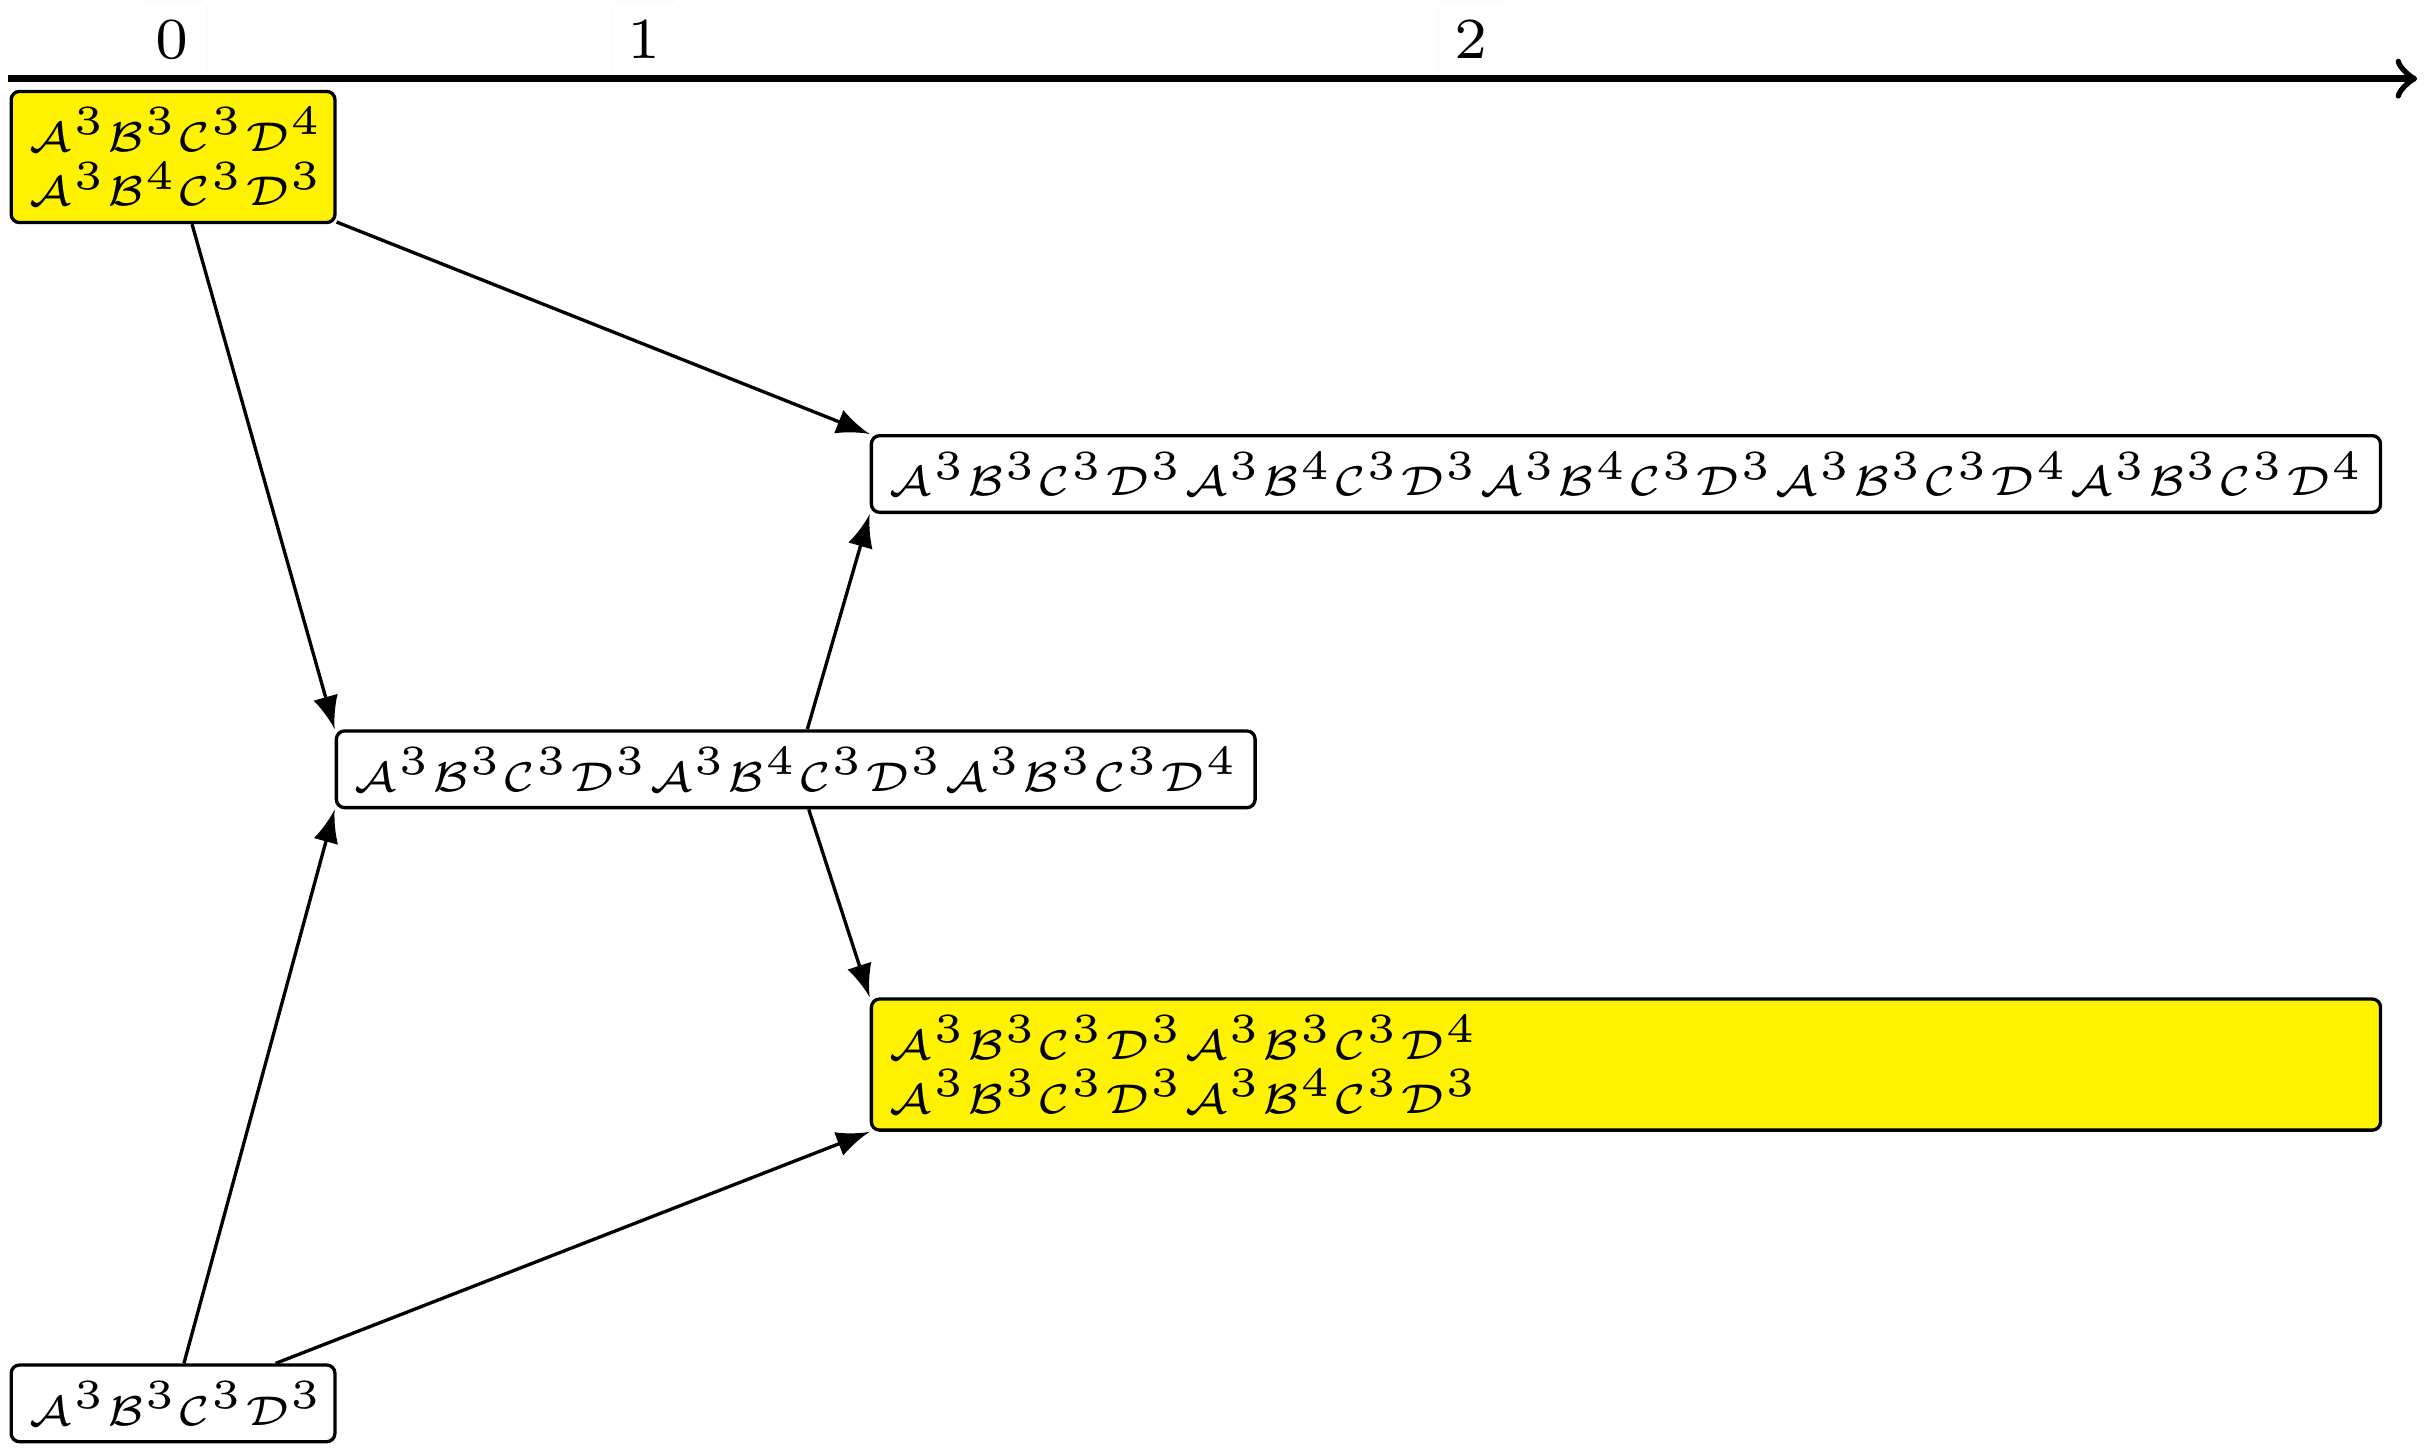
\includegraphics[width=.7 \textwidth]{../Figures/7/7.15+17/adding.png}
	\caption[Farey-tree with the symbolic sequences of a horizontal \glsentrylong{pal} structure]{
		Farey-tree with the symbolic sequences associated with the parameter regions of the left vertical \gls{pal} structure marked with a red arrow in \Cref{fig:add.add.like.vert.2D} up to two levels.
		Nodes of parameter regions associated with two coexisting cycles are colored yellow.
	}
	\label{fig:add.add.like.vert.tree}
\end{figure}

\subsubsection{Period-adding-like Structures in the Corners}

Finally, the structure in the corner which \Cref{fig:add.add.like.corn.2D} shows a 2D period scan of is examined.
Here, we see many \gls{pal} structures.
These are organized as follows.
There is one horizontally oriented \gls{pal} structure between the parameter regions $\left[P^{12}_2 \mid P^{14}_3\right]$ and $P^{12}_3$.
And one horizontally oriented \gls{pal} structure between the parameter region $P^{12}_3$ and every parameter region in the vertically oriented \gls{pal} structure between the parameter regions $P^{12}_2$ and $\left[P^{12}_2 \mid P^{14}_3\right]$.
Analogously, there is one vertically oriented \gls{pal} structure between the parameter regions $P^{12}_2$ and $\left[P^{14}_3 \mid P^{12}_3\right]$.
And one vertically oriented \gls{pal} structure between the parameter region $P^{12}_2$ and every parameter region in the horizontally oriented \gls{pal} structure between the parameter regions $P^{14}_3$ and $\left[P^{14}_3 \mid P^{12}_3\right]$.
Similarly, there is also one horizontally oriented \gls{pal} structure between the parameter region $\left[P^{14}_3 \mid P^{12}_3\right]$ and every parameter region in the vertically oriented \gls{pal} structure between the parameter regions $\left[P^{12}_2 \mid P^{14}_3\right]$ and $P^{14}_3$.
And one vertically oriented \gls{pal} structure between the parameter region $\left[P^{12}_2 \mid P^{14}_3\right]$ and every parameter region in the horizontally oriented \gls{pal} structure between the parameter regions $P^{14}_3$ and $\left[P^{14}_3 \mid P^{12}_3\right]$.
A very similar phenomenon was discovered by \Citeauthor{tramontana2012period} where there are many \gls{pa} structures between some parameter region and every parameter region of a \gls{pa} structure~\cite{tramontana2012period}.

The 1D period scan in \Cref{fig:add.add.like.corn.1D} shows a 1D period scan of one of the simpler \gls{pal} structures.
It is the \gls{pal} structure between the parameter regions $P^{12}_2$ and $\left[P^{14}_3 \mid P^{12}_3\right]$ marked with a red arrow in \Cref{fig:add.add.like.corn.2D}.
The diagram looks exactly like the 1D period scan for the vertical \gls{pal} structure in \Cref{fig:add.add.like.vert.1D}.
Here, the periods also do not add up as we expect them to in \gls{pa} structures.

\begin{figure}
	\centering
	\subfloat[2D period scan]{
		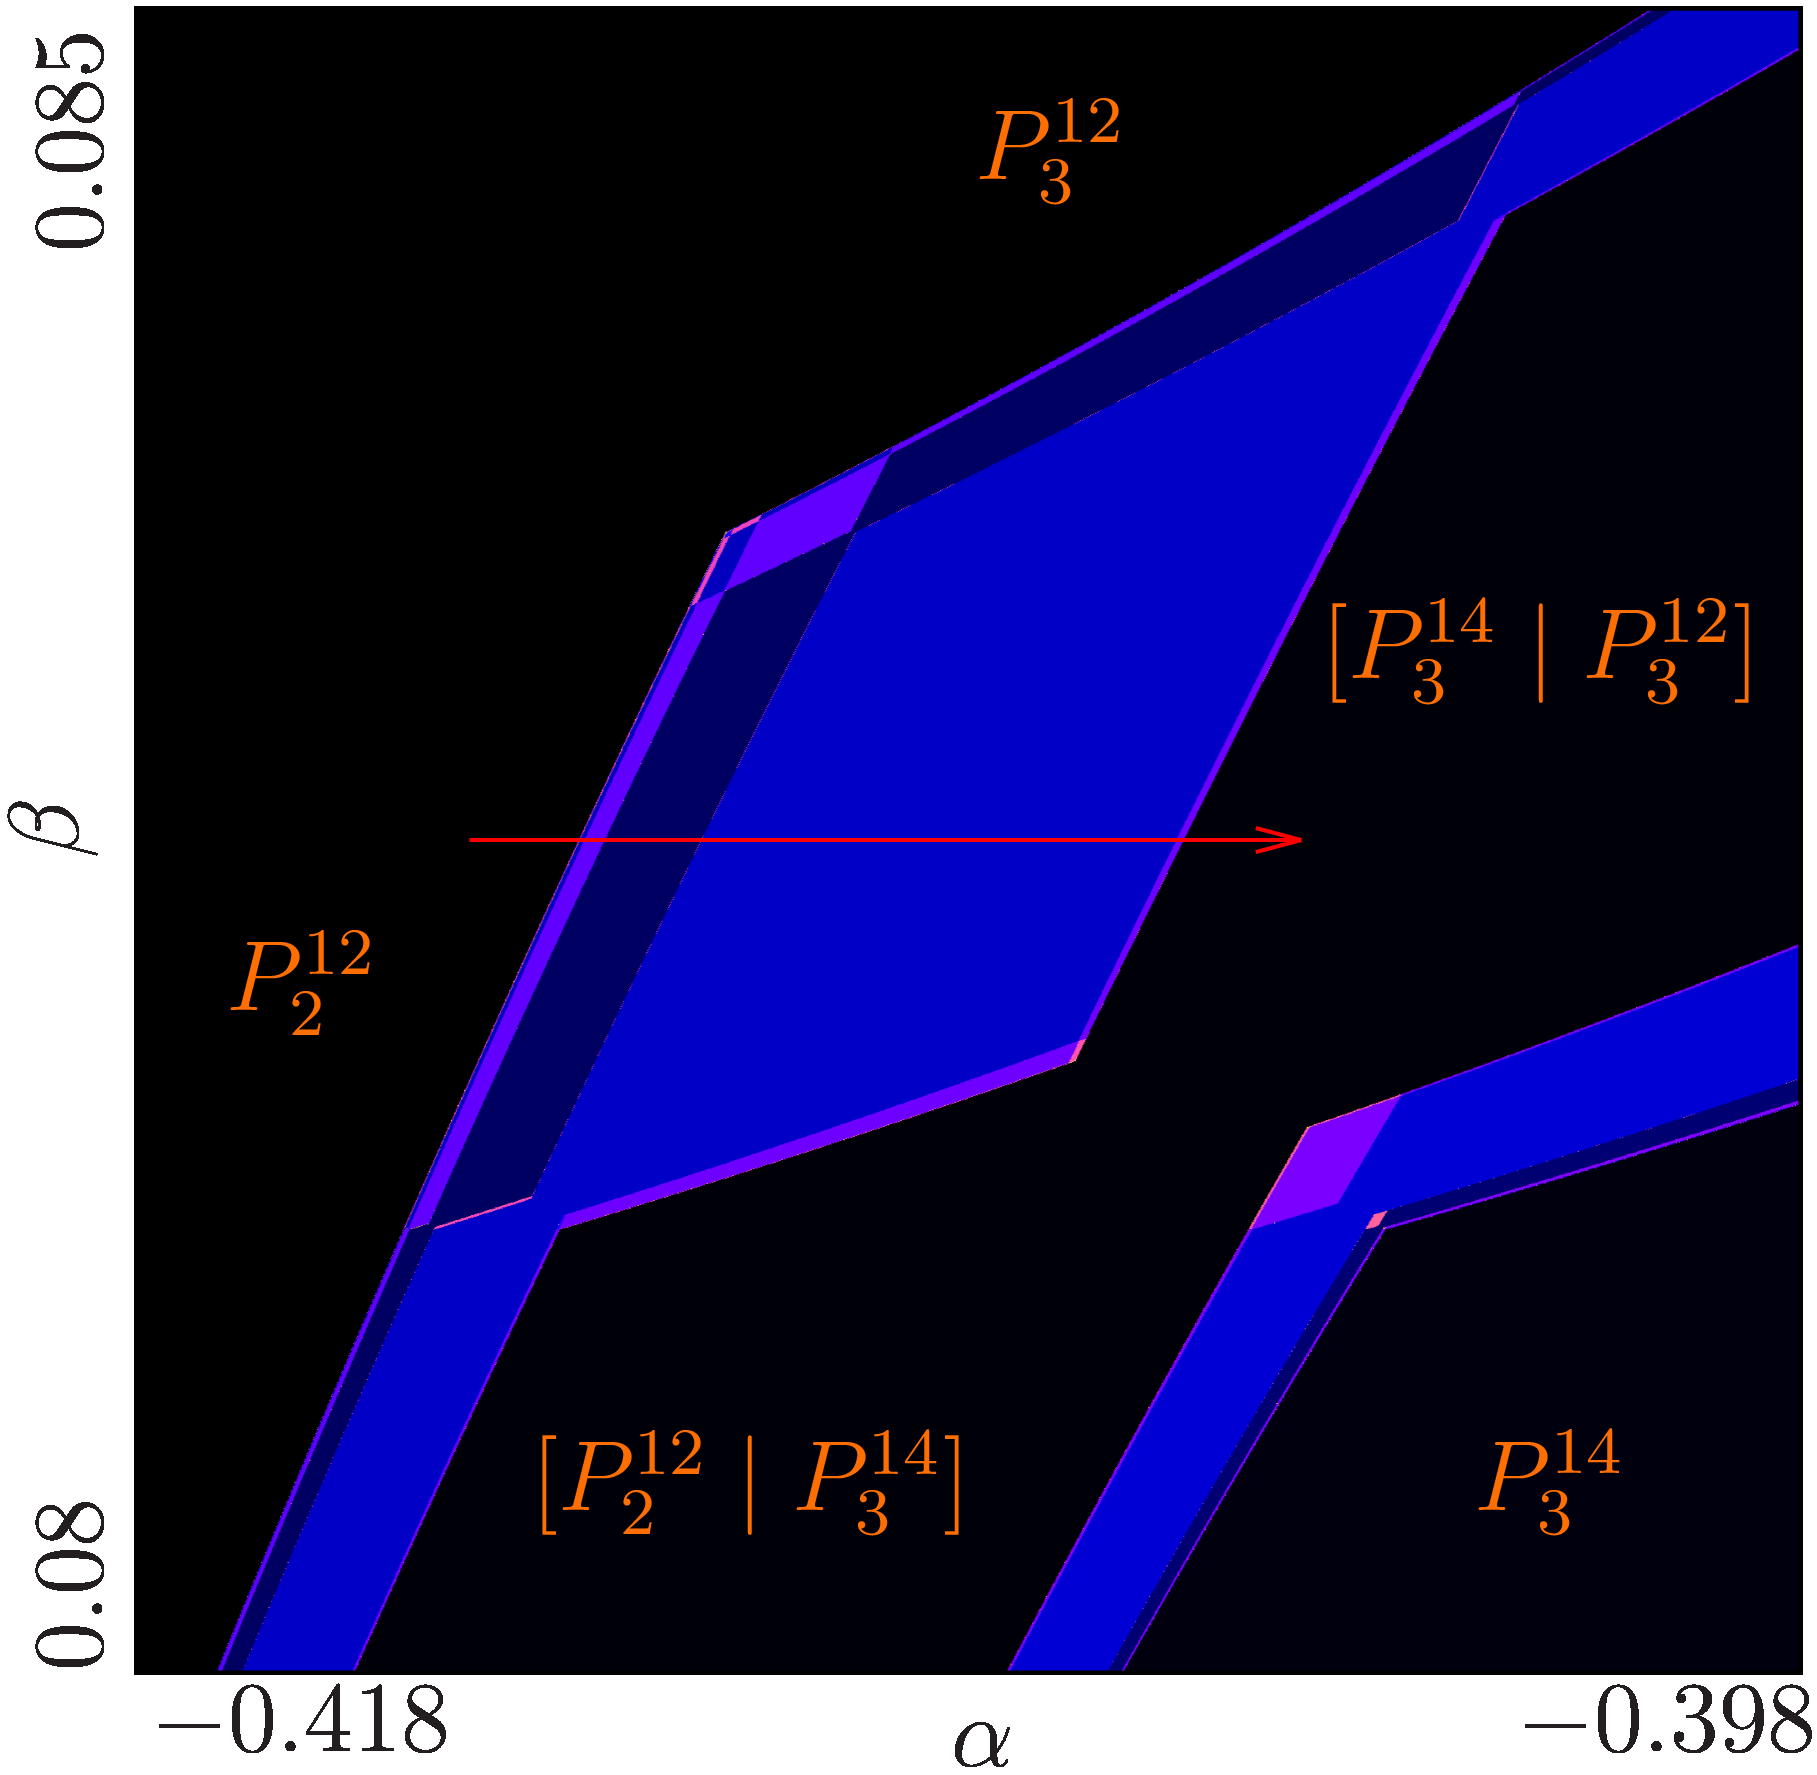
\includegraphics[width=.45 \textwidth]{../Figures/7/7.16a/result.png}
		\label{fig:add.add.like.corn.2D}
	}
	\subfloat[1D period scan]{
		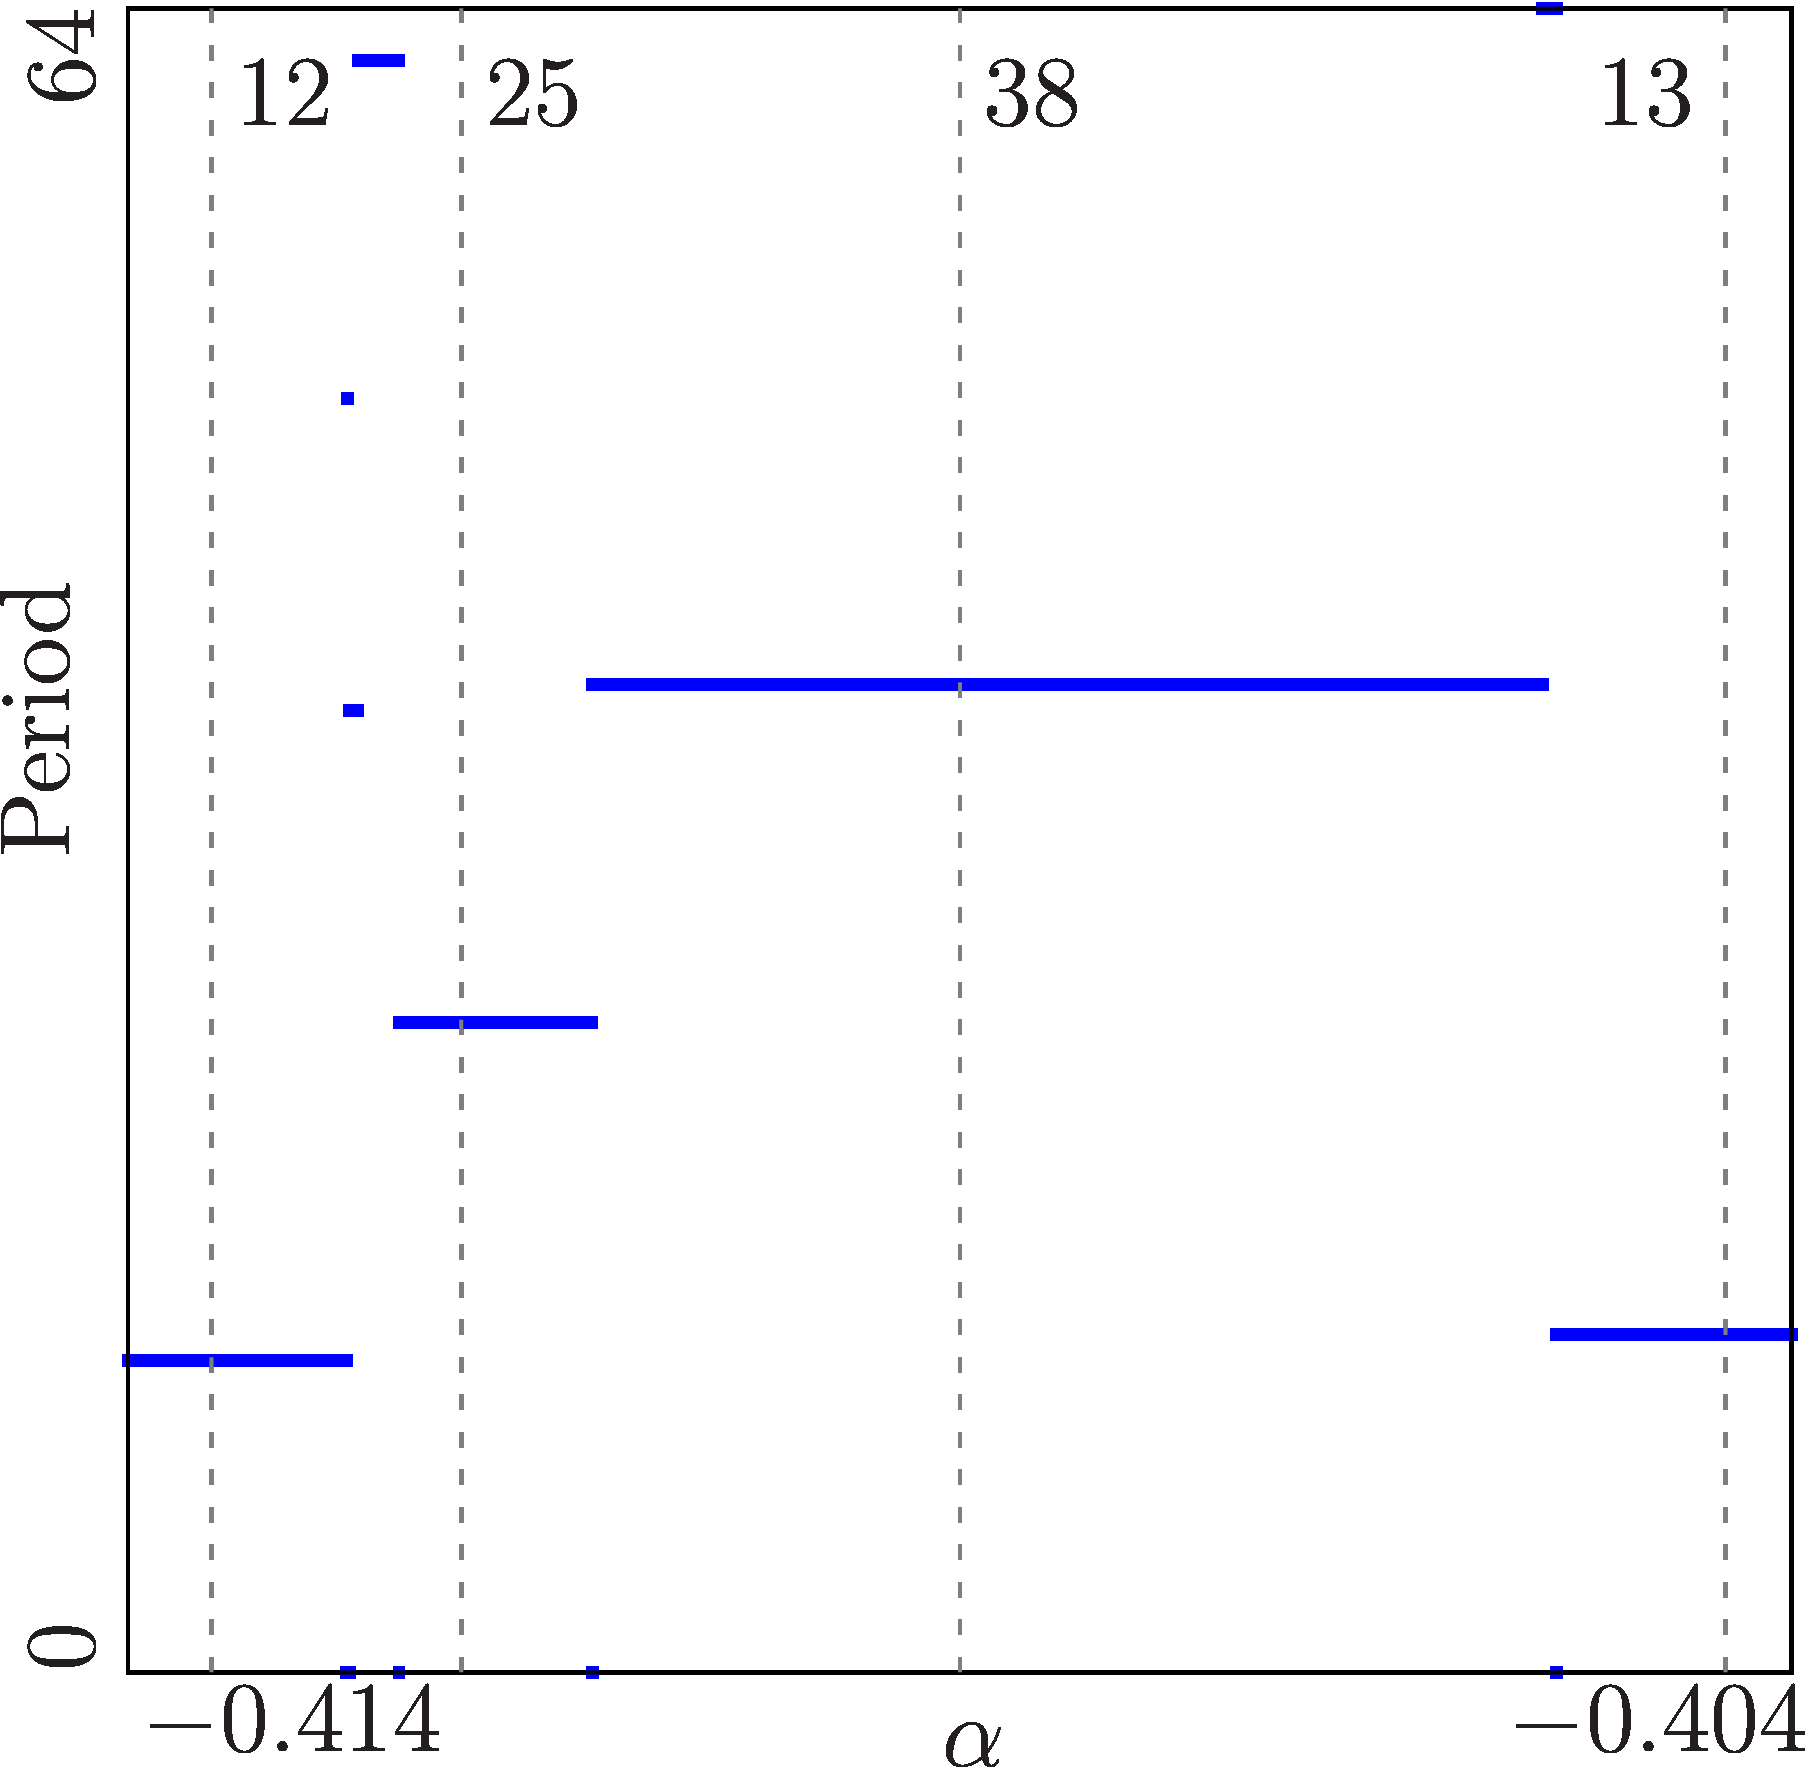
\includegraphics[width=.45 \textwidth]{../Figures/7/7.16b/result.png}
		\label{fig:add.add.like.corn.1D}
	}
	\caption[2D and 1D period scans of period-adding-like structures in the corners of the spaces between chains in the increasing archetypal model]{
		2D and 1D period scans of the period-adding-like structures in the corners of the spaces between chains in the increasing archetypal model.
		The fixed parameters are $a_L = 1, b_L = 0.8,$ and $g_R\left(\frac{1}{2}\right) = \frac{1}{2} + \frac{1}{40}$.
		(a) shows the 2D period scan where the parameters $\alpha = g_R\left(\frac{1}{4}\right)$ and $\beta = c_L$ are varied.
		The big arrow indicates the parameter range for the 1D period scan in (b).
		Here, only $\alpha$ is varied.
		The numbers at the top mark the periods at the corresponding value for $\alpha$.
	}
	\label{fig:add.add.like.corn}
\end{figure}

The symbolic sequences are different from the vertical \gls{pal} structure in \Cref{fig:add.add.like.vert.2D}.
Still the same argument as before works that this structure is not a skewed \gls{pa} structure.
Since there are infinitely many \gls{pal} structures in this corner it is very hard to describe each one and construct rules for the periods and symbolic sequences in the structures.
Luckily there is an easier way to describe the \gls{pal} structures in the increasing archetypal model and construct the wanted rules.
This involves the halved archetypal model, which is introduced in the next section.

\begin{figure}
	\centering
	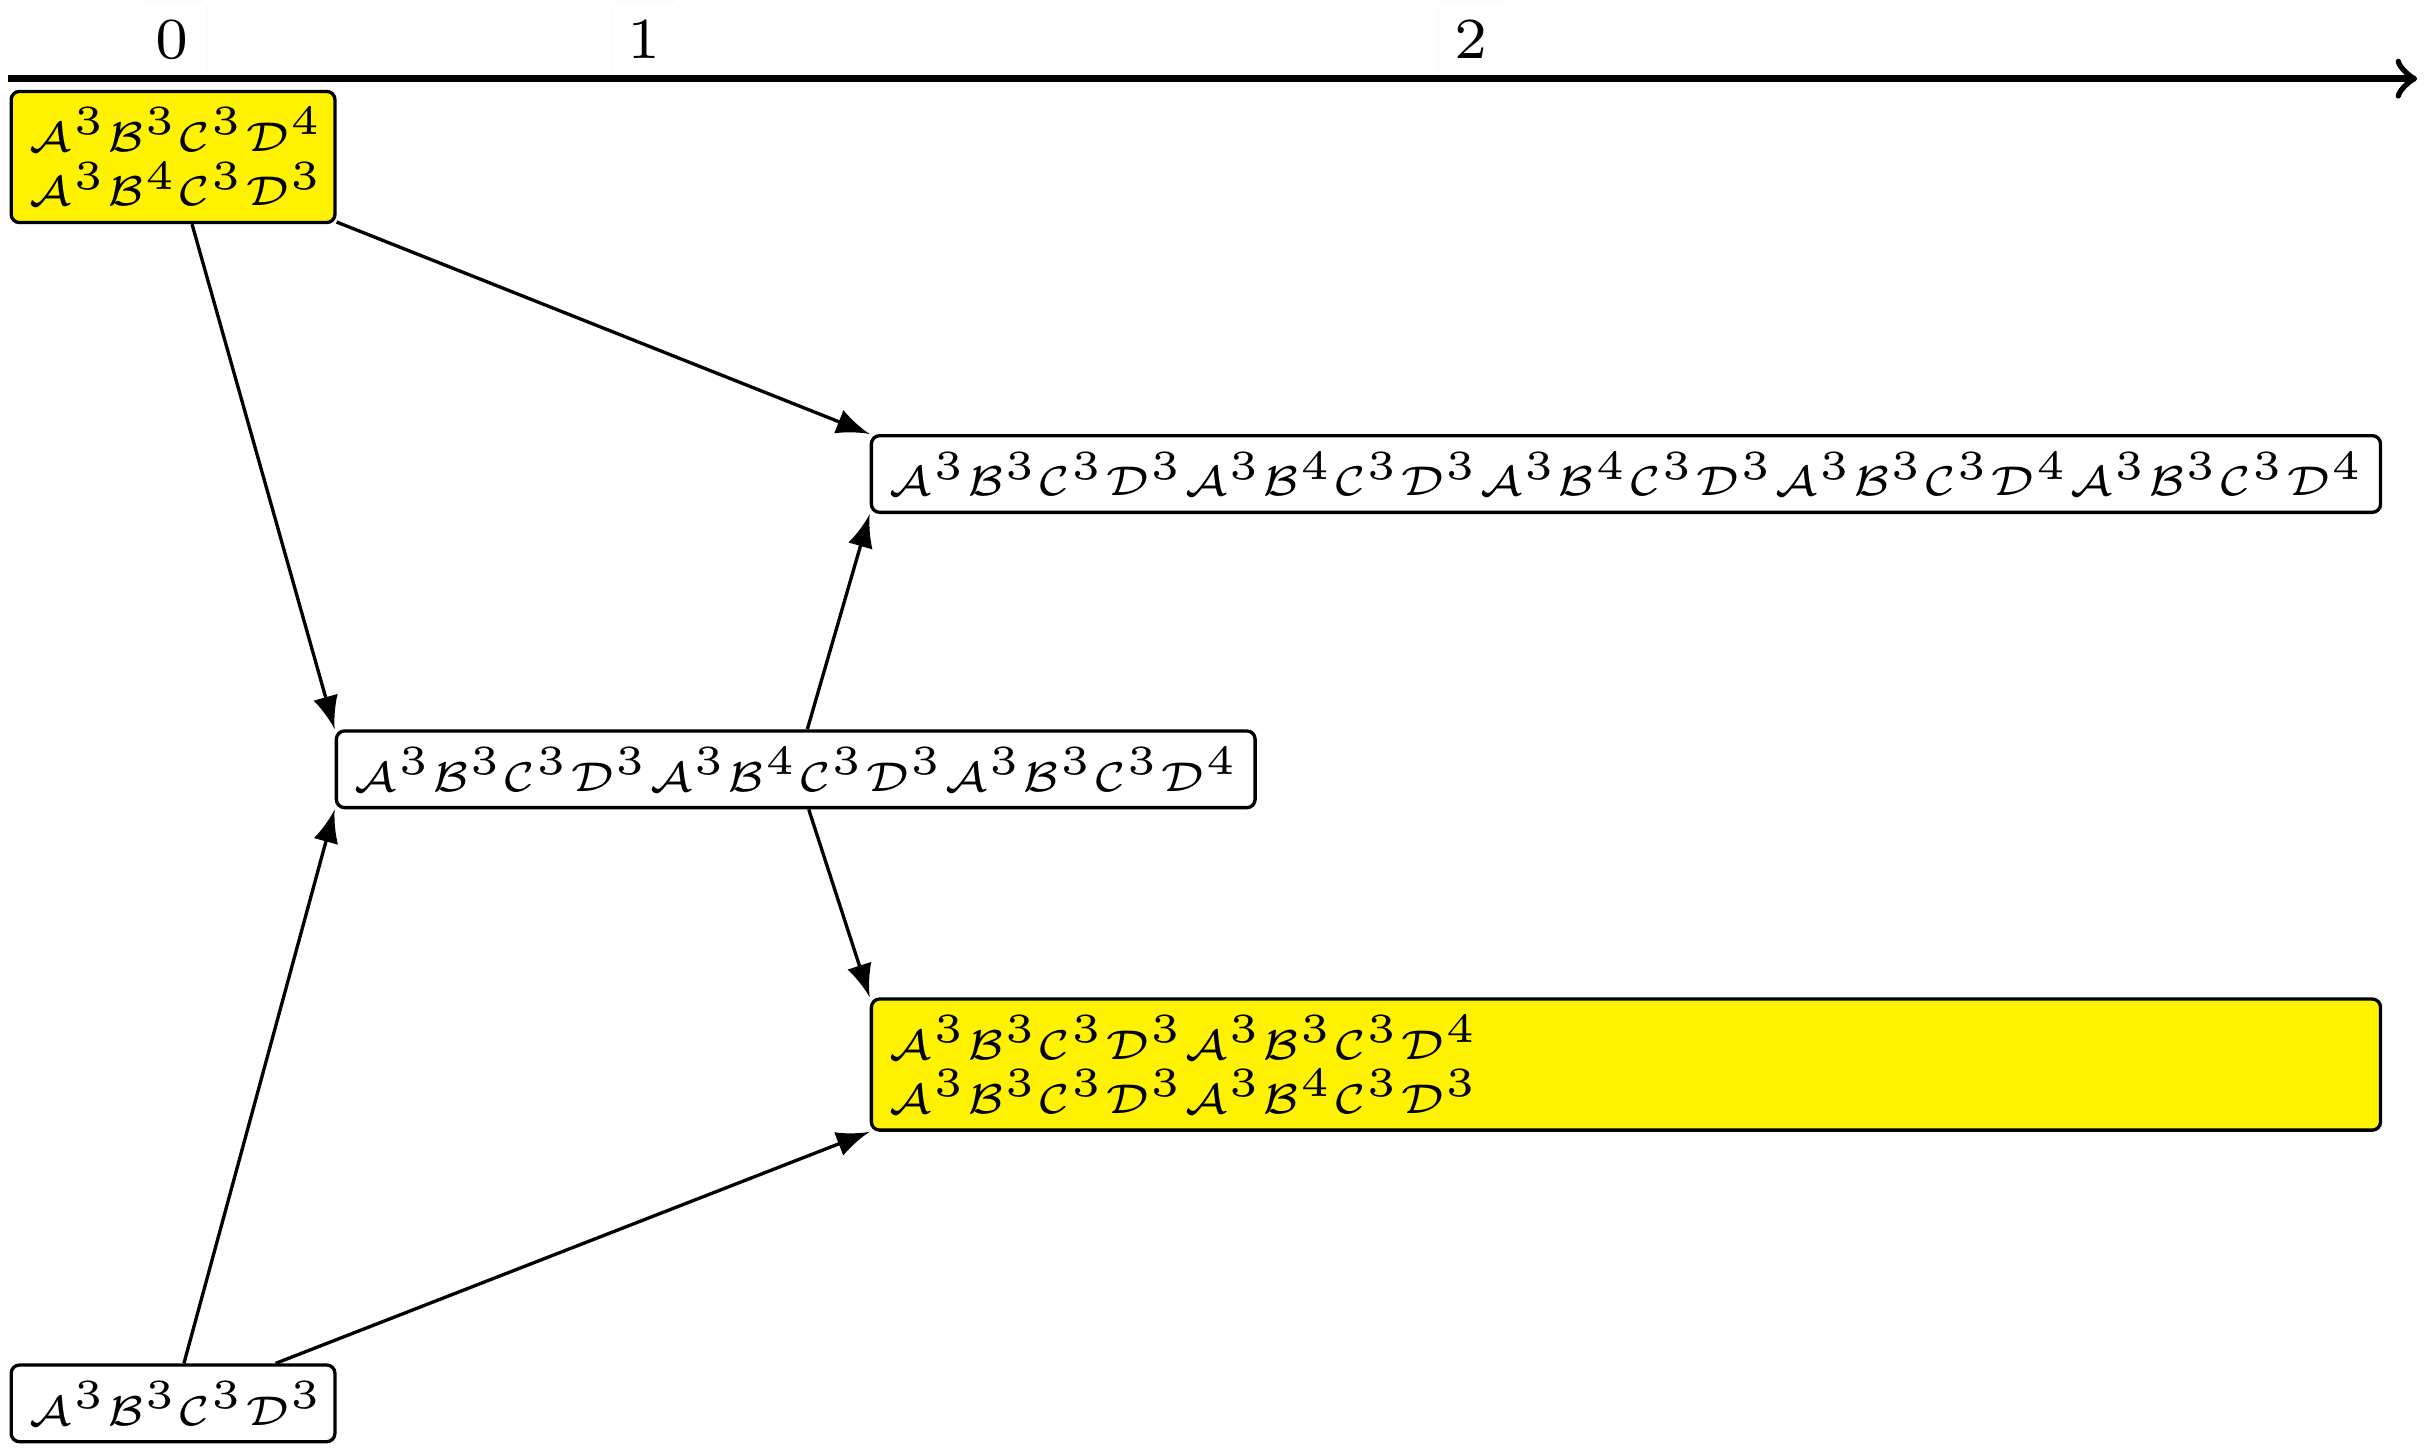
\includegraphics[width=.7 \textwidth]{../Figures/7/7.15+17/adding.png}
	\caption[Farey-tree with the symbolic sequences of a vertical \glsentrylong{pal} structure]{
		Farey-tree with the symbolic sequences associated with the parameter regions of the vertical \gls{pal} structure marked with a red arrow in \Cref{fig:add.add.like.corn.2D} up to two levels.
		Nodes of parameter regions associated with two coexisting cycles are colored yellow.
	}
	\label{fig:add.add.like.corn.vert.tree}
\end{figure}
